%	Copyright (C) 2013 Systems Engineering Group
%
%	CHANGELOG:
%       2005-10-10 - corrected and extended. 
%       2013-01-28 - adjusted sections and explanation
% 	Author: Subramanya Joshi


\documentclass[a4paper,10pt,twoside]{article}
\pagestyle{headings}
\usepackage{a4wide}
\usepackage[english]{babel}
\usepackage{amsmath}
\usepackage{graphicx}
\usepackage[colorlinks,hyperfigures,backref,bookmarks,draft=false]{hyperref}
\usepackage{listings}

\title{Analysis of migration time of live migration of VM's running benchmarks from a subset of SPEC CPU2006 benchmark suite}
\author{Subramanya Joshi
\\ Supervisor: M.Sc. Kateryna Rybina \\
TU Dresden}
\date{30.04.2015}

\begin{document}

\maketitle

\begin{abstract}
Live migration \cite{clark2005live} is a process of transferring the execution of virtual machines (VM's) from one host to another without stoping the execution of the VM or any workload running inside the VM. Migration of the VM  can be used to consolidate the workload on a small set of host servers, allowing for rapid elasticity without compromising the availability. In the process of  live migration the user workload running inside the VM's will not be interrupted, hence making the process transparent to the end-user. This process of  VM migration incurs an overhead  cost on the source and destination host servers. Such costs are migration time, increases time of execution of user tasks, power consumption etc \cite{strunk2013does}. In this Internship, I have carried out a study on the impact of various parameters like page dirty rate, last level cache misses, RAM utilisation, network bandwidth and Memory access rate in ten SPEC2006 benchmarks on migration time \cite{rybina2014analysing}. 
\end{abstract}

\tableofcontents
\section{Assigned Task}
\begin{enumerate}
 \item Get familiar with the state-of-the-art papers concerning the live migration of the VM's and modelling the VM migration time.
 \item Select 10 sub-benchmarks from SPEC CPU2006 benchmark suite (5 CPU intensive and 5 memory intensive), run them as the workload on the VM's during live VM migration. 
 \item Realise the VM migration varying the available for migration bandwidth from 70 MBps to 100 MBps in steps of 10 MBps.
 \item Estimate the execution time of benchmarks with and without the live migration of the VMs. Quantify the service degradation.
 \item As suggested by the supervisor test the concept, namely how the migration time of the VM's depends on the system parameters such as: 1) memory page dirty rate, 2) last level cache miss rate 3) cpu utilisation, 4) RAM utilisation, 5) available for migration network bandwidth etc.
 \item Model these dependencies using multiple linear regression technique.
 \item Include only significant parameters in the model which can be used to predict migration time.
\end{enumerate}
\section{Introduction}
Server virtulization technology has recently emerged as essence of data centres and cloud computing systems, mainly due to its capabilities of isolating, consolidating and migrating workload. Altogether, these features allow a data centre to serve multiple users in a secure, flexible and efficient way. Consequently, these virtualized infrastructures are considered as a key component to drive the emerging Cloud Computing paradigm \cite{voorsluys2009cost}. \\
Migration of the VM's  can be used to consolidate the workload on a small set of host servers, allowing for rapid elasticity without compromising the availability. The ability to migrate an entire operating system overcomes most difficulties that traditionally have made process-level migration a complex operation. The applications themselves and their corresponding processes do not need to be aware that a migration is occurring. Hypervisors, such KVM, allow migrating an OS as it continues to run. Such procedure is termed as live or hot migration, as opposed to pure stop-and-copy or cold migration, which involves halting the VM, copying all its memory pages to the destination host and then restarting the new VM. The main advantage of live migration is the possibility to migrate an OS with near-zero downtime, an important feature when live services are being served.\cite{habib2008virtualization}
\section{Concept suggested by the supervisor}
Process of live VM migration increases the resource consumption on both source and destination machines. This process of live migration of VM has significant influence on CPU utilisation, CPU cache hit-miss, memory utilisation , network bandwidth utilisation and power consumption of the hosts. As suggested by my supervisor, I carried out the experiment by creating the VM with SPEC2006 sub benchmarks executing within the VM (List of subset of benchmark considered at listed in Table-1) and recording the various parameters (List of various parameters recorded are listed in Table-2) of resource consumption during the process of live migration of the VM. In the following section I will describe the details of the Workload , Experiment setup, dataset acquired  from the experiments and linear regression models which could be used to explain the dataset.
\section{Workload and Benchmark}
In this experiment I illustrate the influencing of various parameter like - page dirty rate, last level cache misses, RAM utilisation, network bandwidth and Memory access rate on determining the VM migration time which is running the workloads from a subset of SPECCPU2006 benchmark.  Based on the study by \cite{jaleel2010memory}, which determine the memory requirements of workloads from the SPEC CPU2000 and SPEC CPU2006 benchmark suites. Based on this study \cite{jaleel2010memory}, choosing ten sub-benchmarks from SPECCPU2006 benchmark suit based on the benchmarks memory and CPU utilisation. These ten sub-benchmarks are divided into CPU Intensive and Memory Intensive benchmarks. A benchmark is CPU Intensive if it has highest Clockticks per Instructions Retired (CPI) \footnote{https://software.intel.com/sites/products/documentation/doclib/iss/2013/amplifier/lin/ug\_docs/GUID-5C38FB45-A3ED-41F2-B57C-2B513A666205.htm} in SPECCPU2006 benchmark suit. A benchmark is Memory Intensive if it has highest CPI as well as higher memory read's-write's. 
Table-1 shows the list of Benchmarks and its characterisation. 
\begin{table}[ht]
\caption{Subset of SPEC2006 benchmark considered for this expirement}
\begin{center}
    \begin{tabular}{ | l | l | p{5cm} | p{5cm} |}
    \hline
    Benchmark Name & Characterisation &  Summary (take from \cite{henning2006spec}) \\ \hline
    zeusmp & CPU Intensive & A computational fluid dynamics 
    code developed at the Laboratory for Computational Astrophysics
     (NCSA, University of Illinois at Urbana- Champaign) for the simulation of astrophysical phenomena. & Floating Point Benchmark. \\ \hline
    gromacs & CPU Intensive  & A versatile package that performs molecular dynamics. & Floating Point Benchmark\\ \hline
    namd & CPU Intensive  & A parallel program for the simulation of large biomolecular systems. & Floating Point Benchmark\\ \hline
    sphinx3 & CPU Intensive  & A speech recognition system from Carnegie Mellon University. & Floating Point Benchmark  \\ \hline
    soplex & CPU Intensive  &  SoPlex solves a linear program using the Simplex algorithm. & Floating Point Benchmark\\ \hline
    mcf & Memory Intensive  & A program used for single-depot vehicle scheduling in public mass transportation. & Integer Benchmark \\ \hline
    GemsFDTD & Memory Intensive  &  solves the Maxwell equations in 3D in the time domain using the finite-difference time-domain (FDTD) method. & Floating Point Benchmark\\ \hline
    omnetpp & Memory Intensive  &  Simulation of a large Ethernet network, based on the OMNeT++ discrete event simulation system, using an ethernet model which is publicly available . & Integer Benchmark\\ \hline
    astar & Memory Intensive  & 2D path-finding library that is used in game's artificial intelligence. & Integer Benchmark\\ \hline
    milc & Memory Intensive  &  Simulations of four dimensional lattice gauge theory on multiple instruction - multiple data parallel systems. & Floating Point Benchmark\\ \hline
    \end{tabular}
\end{center}
\label{tab:gt}
\end{table}
\section{Experiment Setup}
The experiment is based on the live migration of virtual machine, which is running a subset of SPECCPU2006 benchmark, from the source physical machine to the destination physical machine using network attached storage (NAS), and the client machine to trigger migration as shown in Figure 1.Two physical machines under test are homogeneous with system configuration of:  Intel 15- 680 Dual Core 3.6 GHz processors, 4 GB DDR3- 1333 SDRAM, and with 1 Gbit/s Ethernet NIC. They are interconnected via a 1 Gbit/s switch. The NAS on which the VM images are located has the following characteristics: Intel Xeon E5620 Quad-Core 2.4 GHz processor, 10 GB DDR3-1333 SDRAM memory, and 1 Gbit/s Ethernet NIC. NAS is always accessed by the source and the destination hosts. \\
Ten sub benchmarks from SPECCPU2006 benchmark suit are executed one after another on the virtual machines. While each benchmark is being executed, VM is migrated from the source to destination server at different network bandwidth like 70 MBps, 80 MBps, 90 MBps and 100 MBps. When the benchmarks are being executing, based on their execution time, a total of ten migrations were performed between the source and destination hosts. \\
During the process of migration various tools are used to measure the system wide resources utilisation. dstat \footnote{http://linux.die.net/man/1/dstat} program on the source and destination servers, as well as VMs was used to observe and record resource utilisation (CPU and memory), Intel Performance counter monitor \cite{knight2004method} program was used to monitor and record the CPU data like - L1,L2 ,L3 hit-miss, CPU temperature, Instructions retired etc. And Page dirty statistics were recorded from Linux Kernal for Source , Destination and VM machines. Before the experiments took place all the servers were time synchronised in order to accurately determine the beginning and the end of a VM migration. Besides the resource utilisation and migration times the power consumption of the two servers was also recorded.
\begin{figure}[h]
\centering
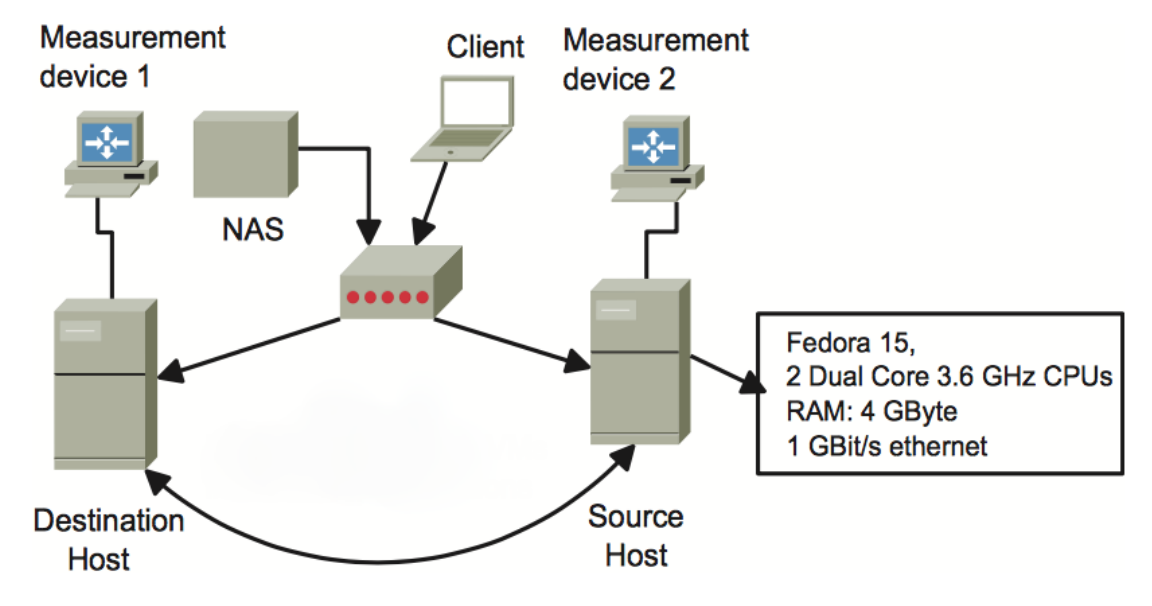
\includegraphics[scale=0.5]{setup.png} 
\caption{Experimental setup for live migration of VM \cite{rybina2013investigation}}
\end{figure}
\section{Results}
Overall, our experimental results show that overhead due to live migration is acceptable but cannot be disregarded. Figure 2 shows the total execution time taken for each benchmark. The figures in the Figure 1 show, time taken for the execution with and without VM migration during the process of execution of the benchmark. Figure 3 shows the time taken for each migration under different bandwidth capacity.
\begin{figure}[h]
\centering
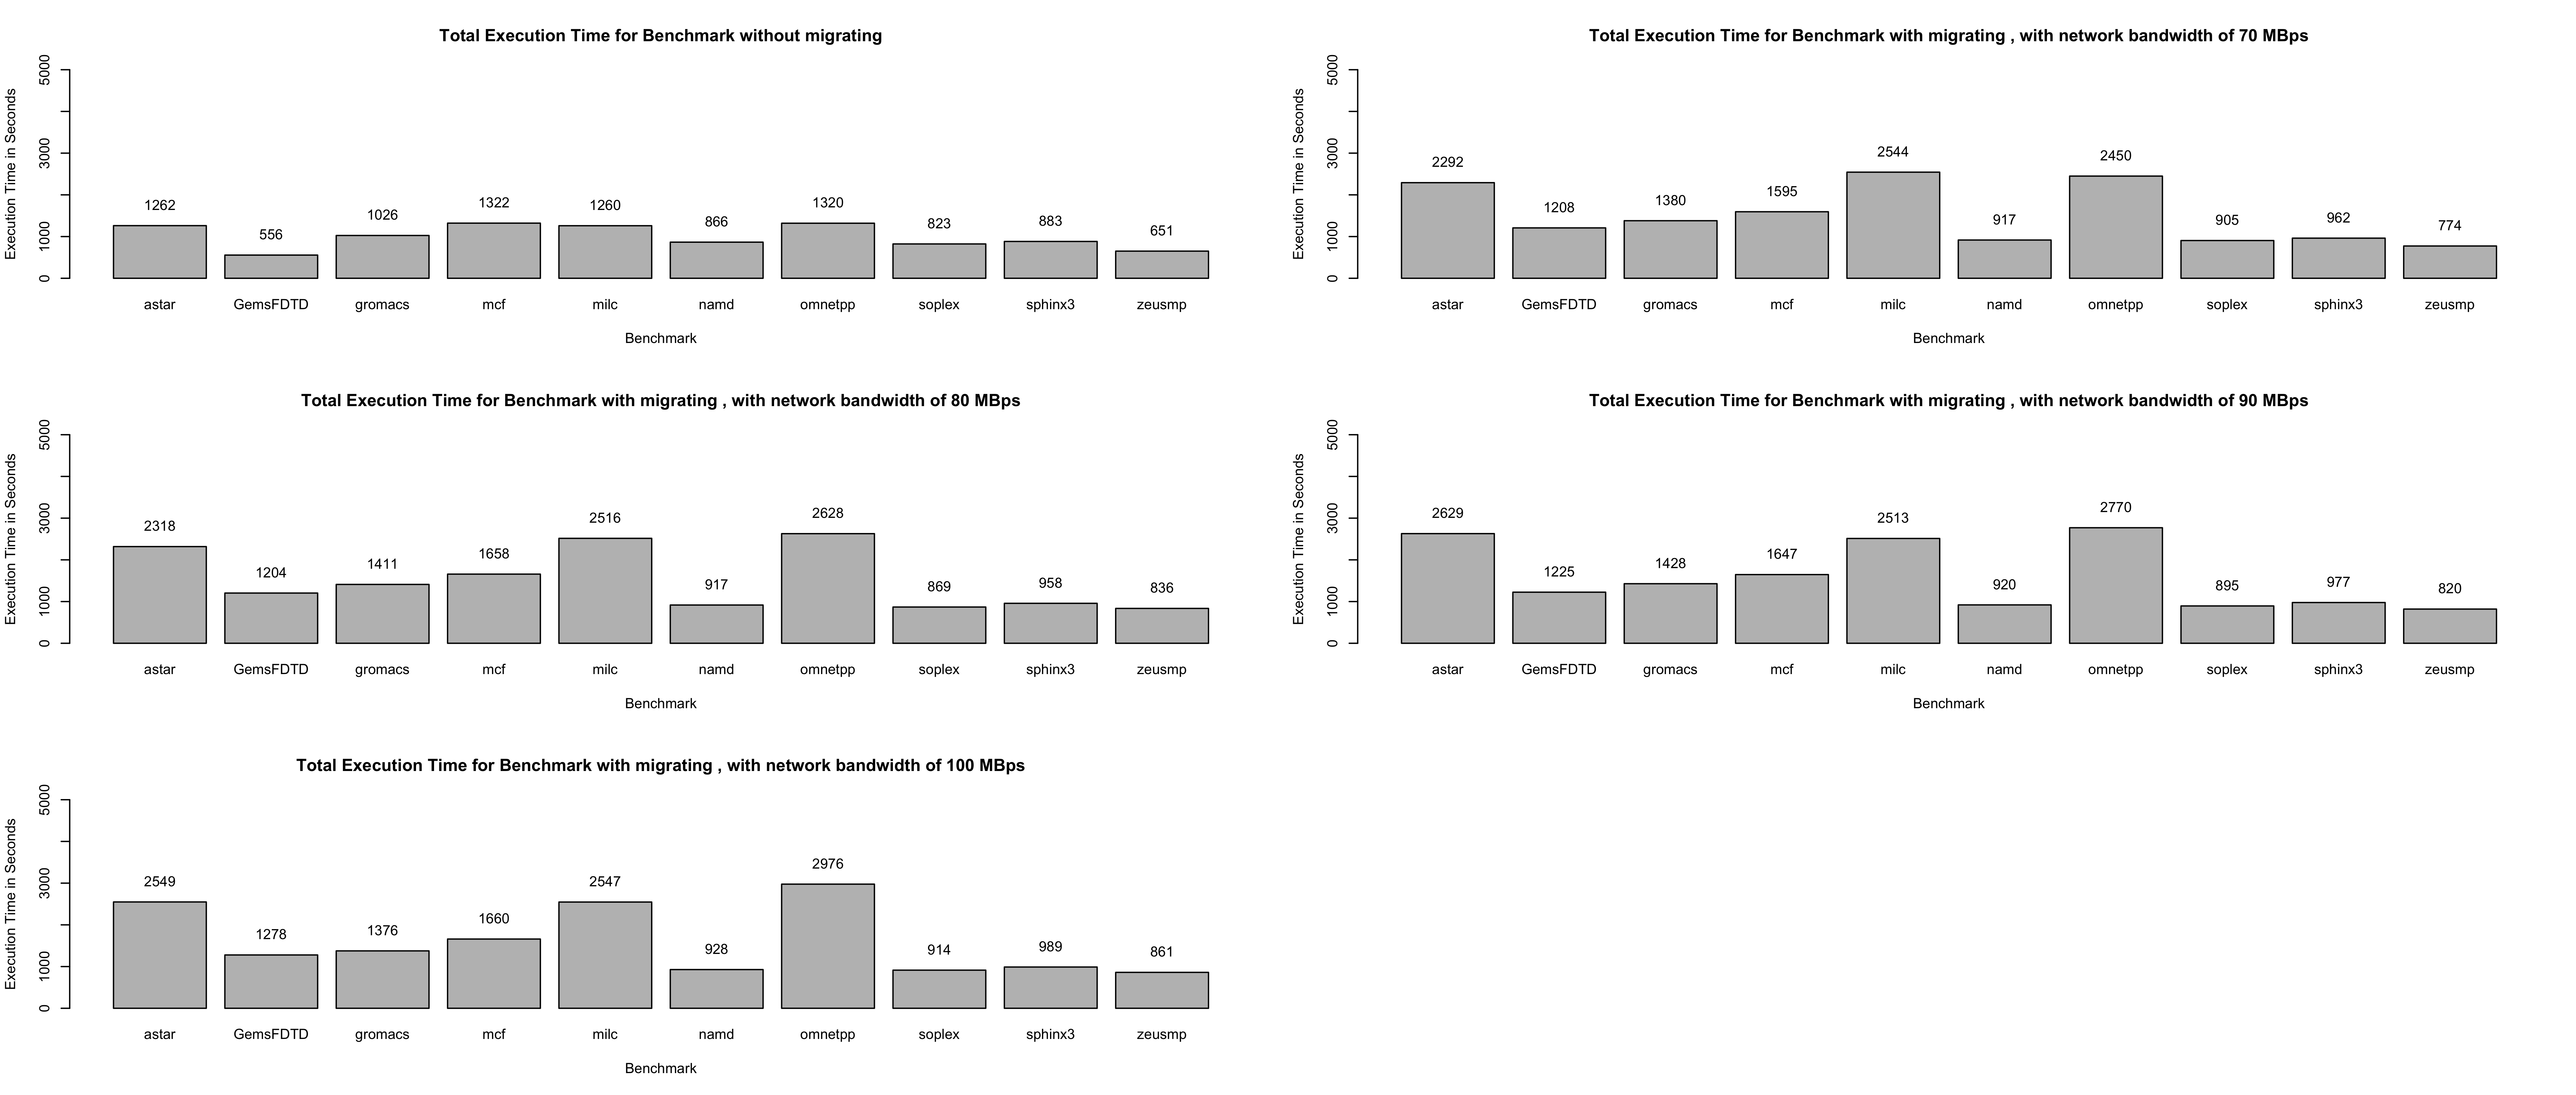
\includegraphics[width=500px]{benchmark_acutal_migrationtime.png} \\ 
\caption{Time taken for execution of benchmarks with and without migration}
\end{figure}

\begin{figure}[h]
\centering
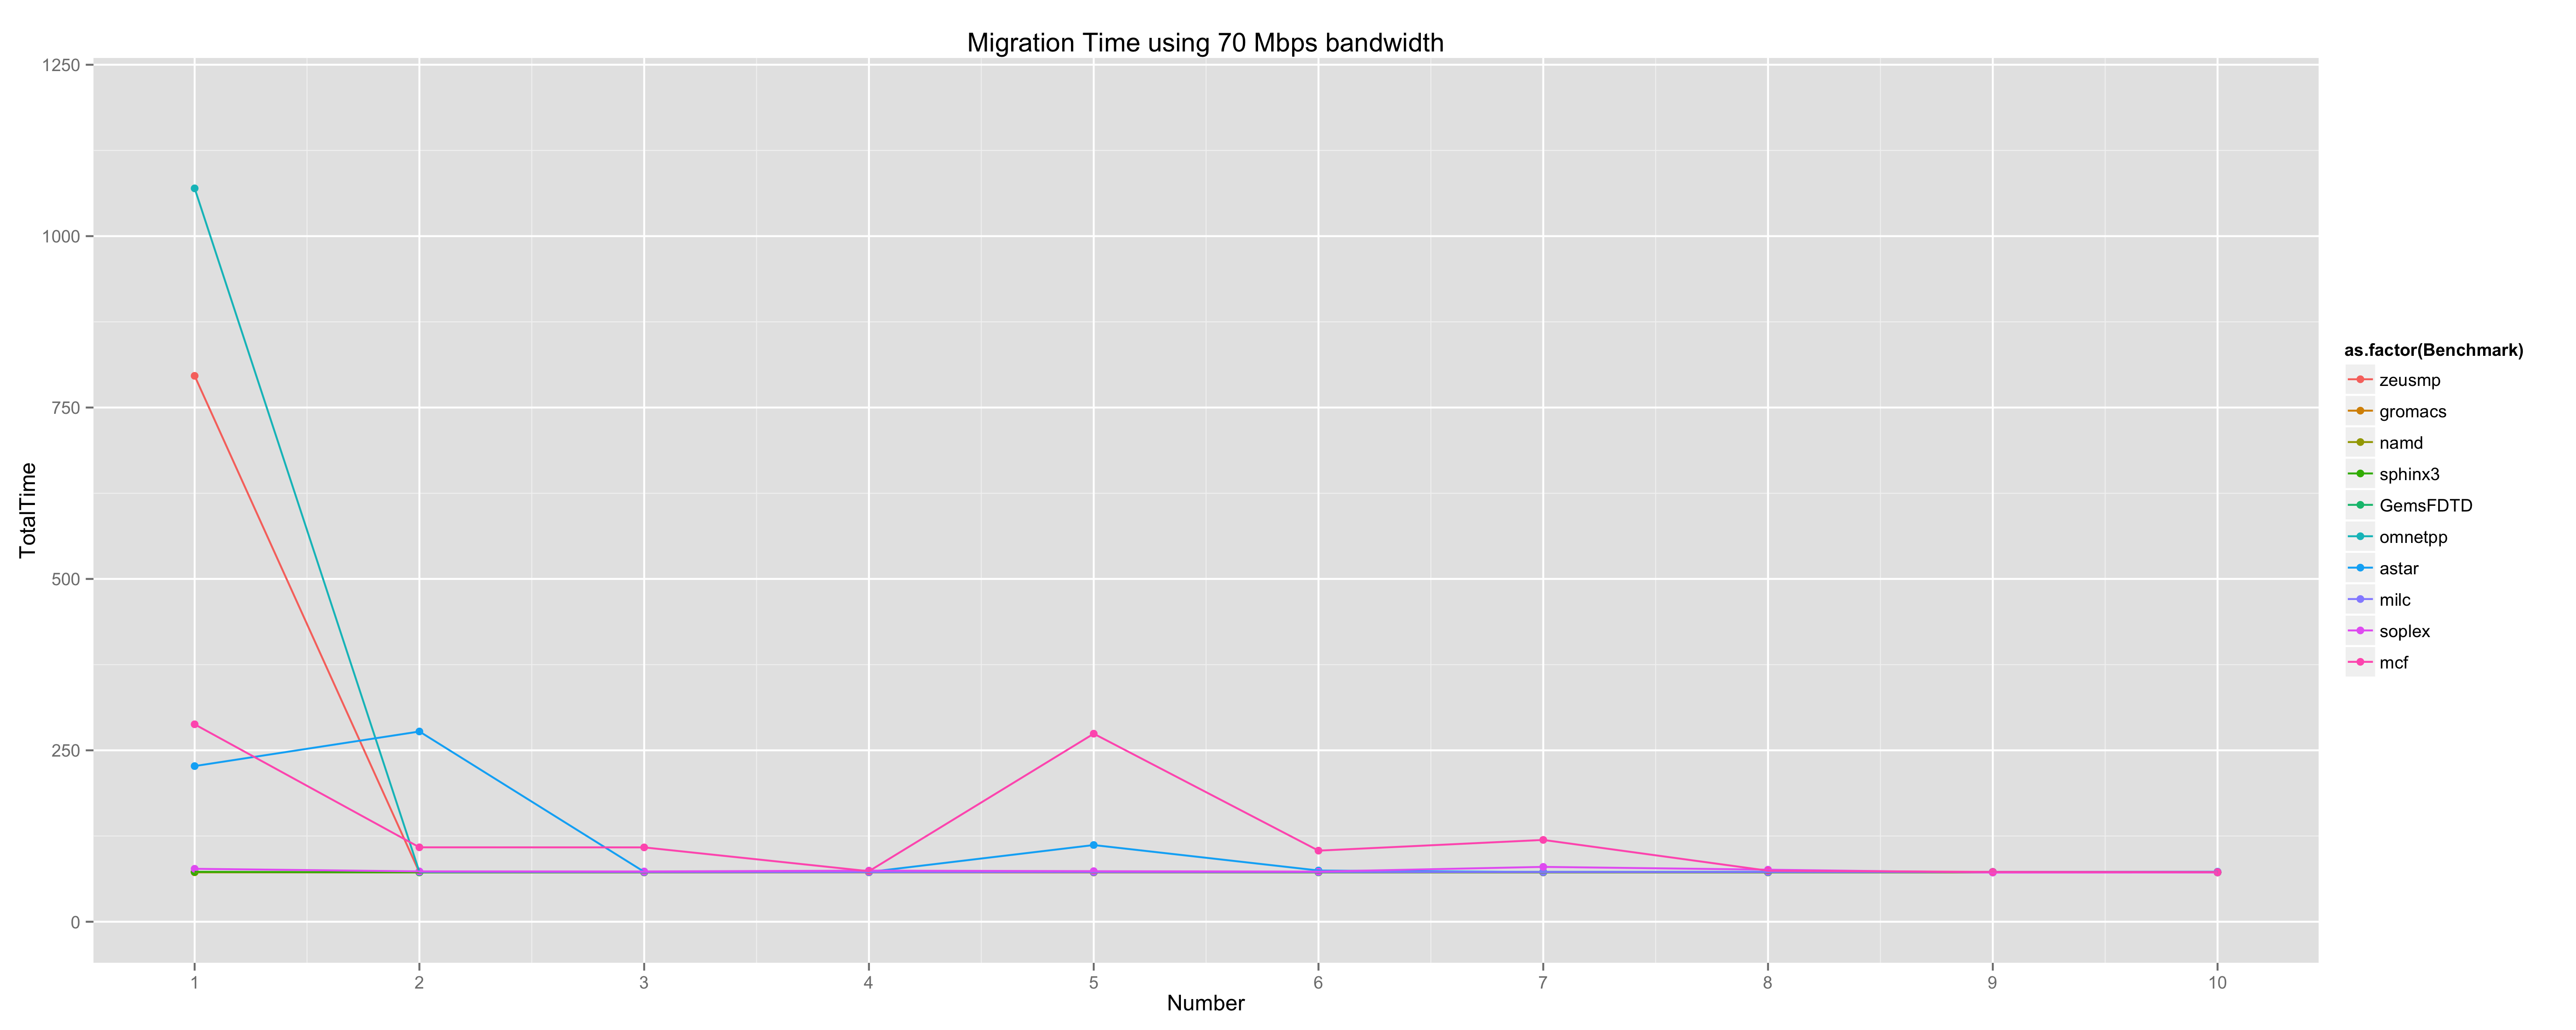
\includegraphics[width=400px]{migration_time70.png} \\ 
 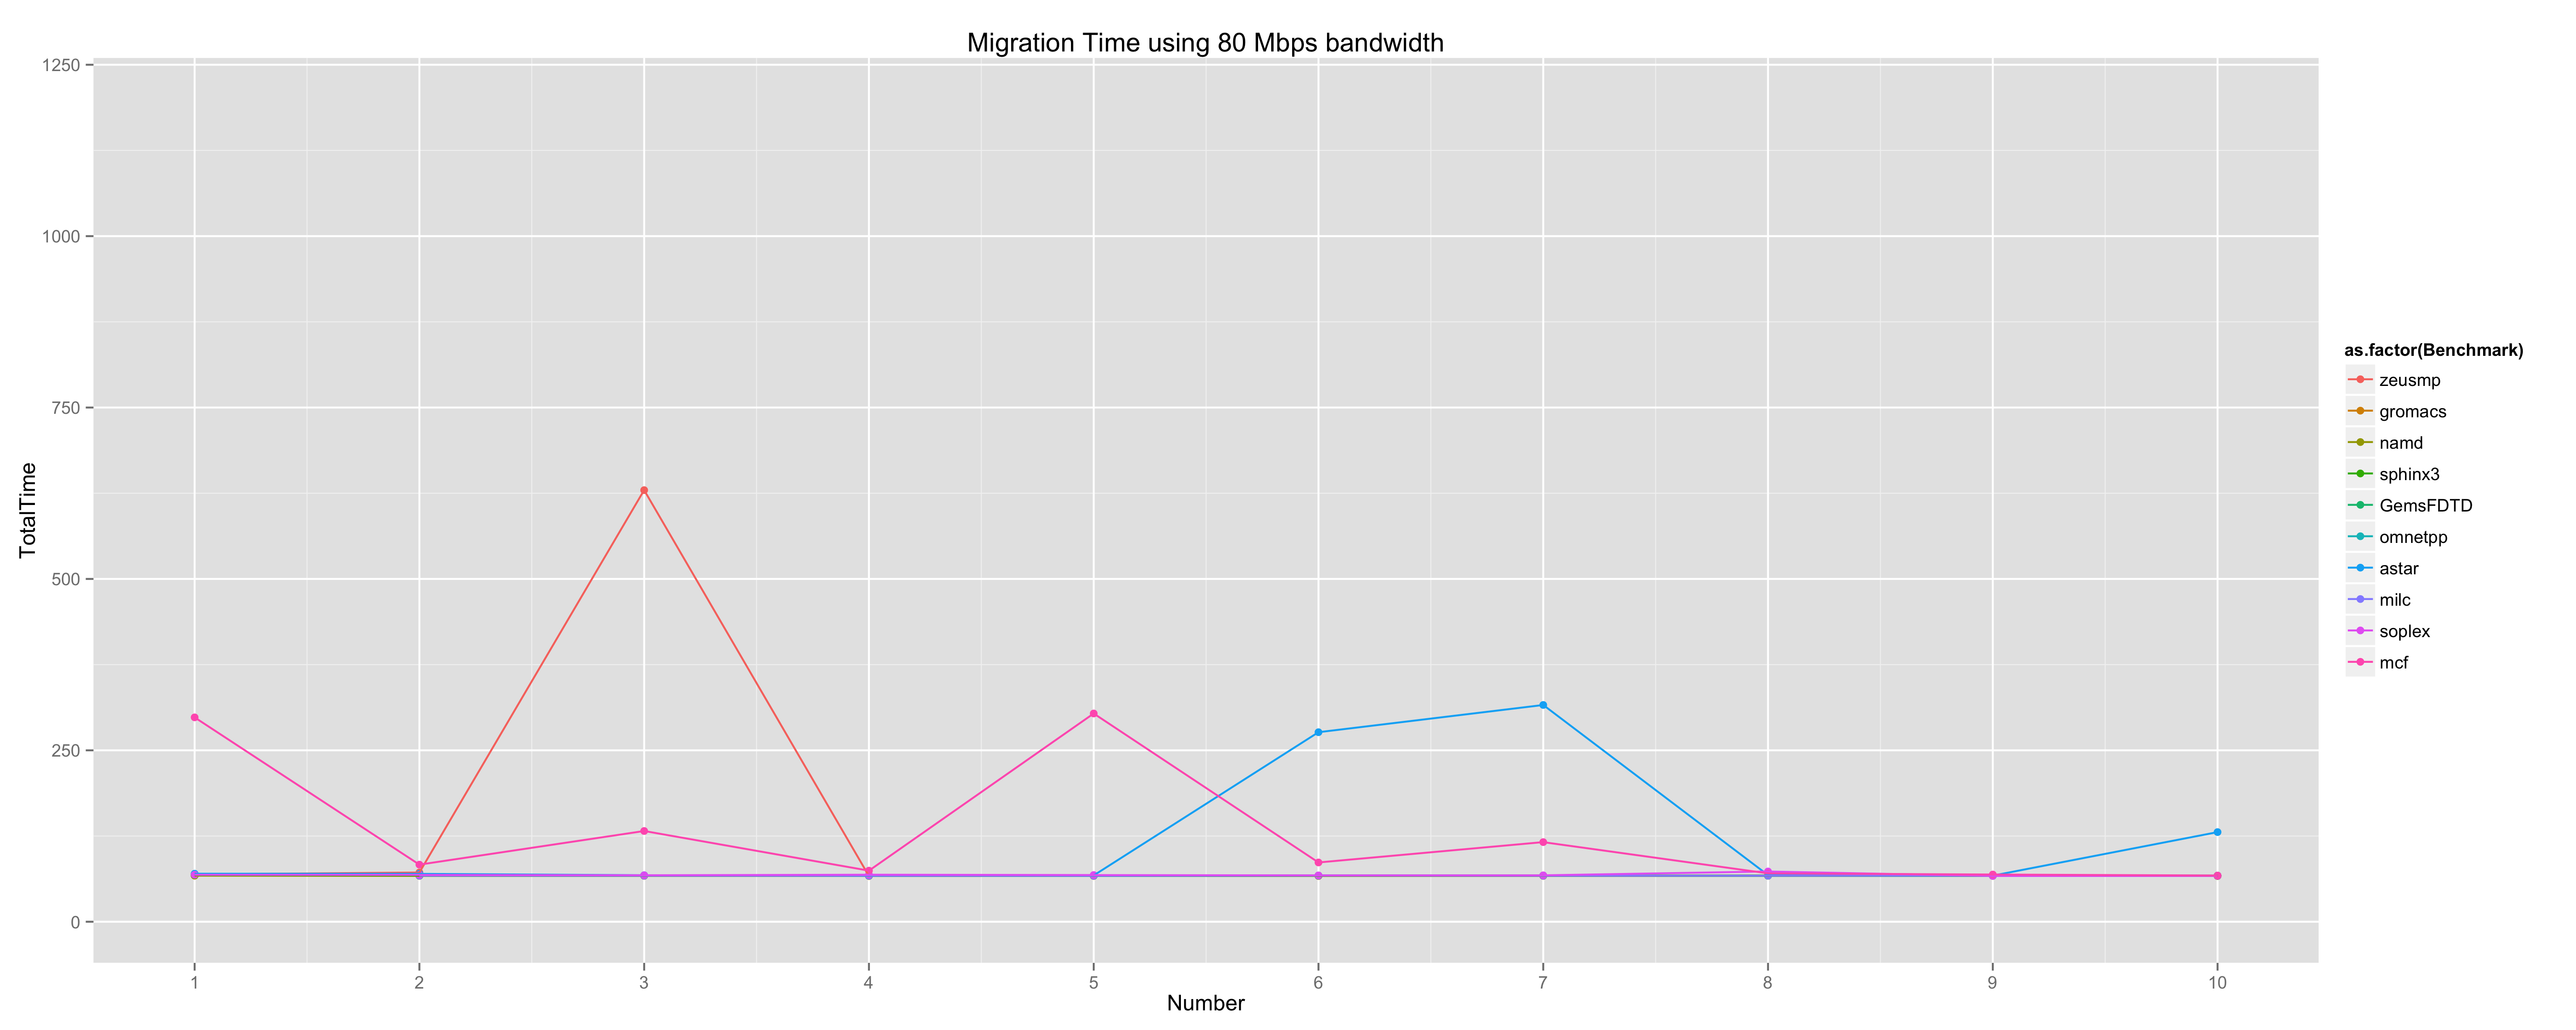
\includegraphics[width=400px]{migration_time80.png}\\  
 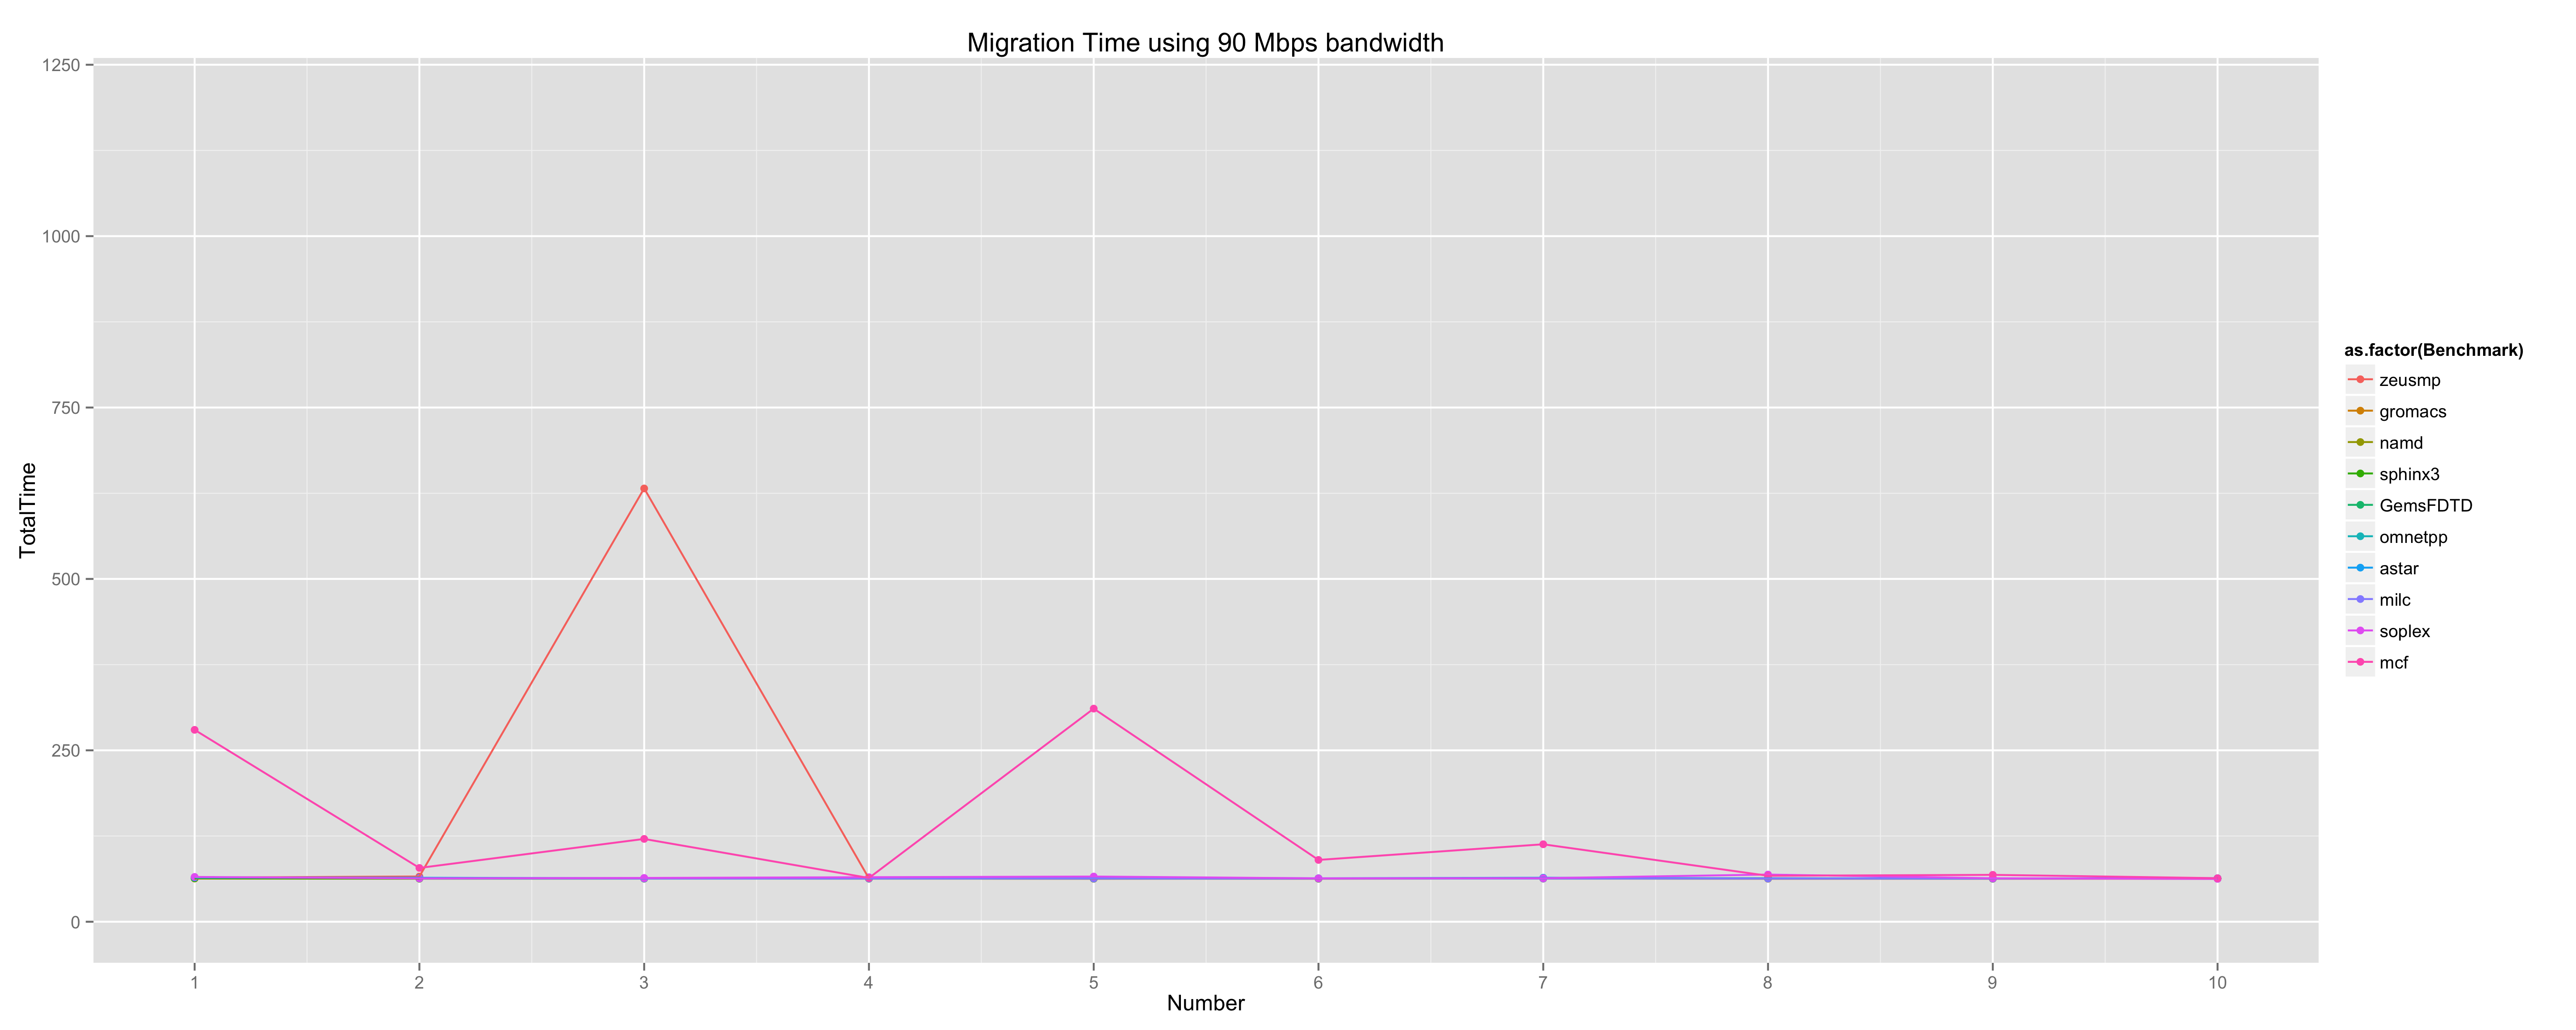
\includegraphics[width=400px]{migration_time90.png} \\ 
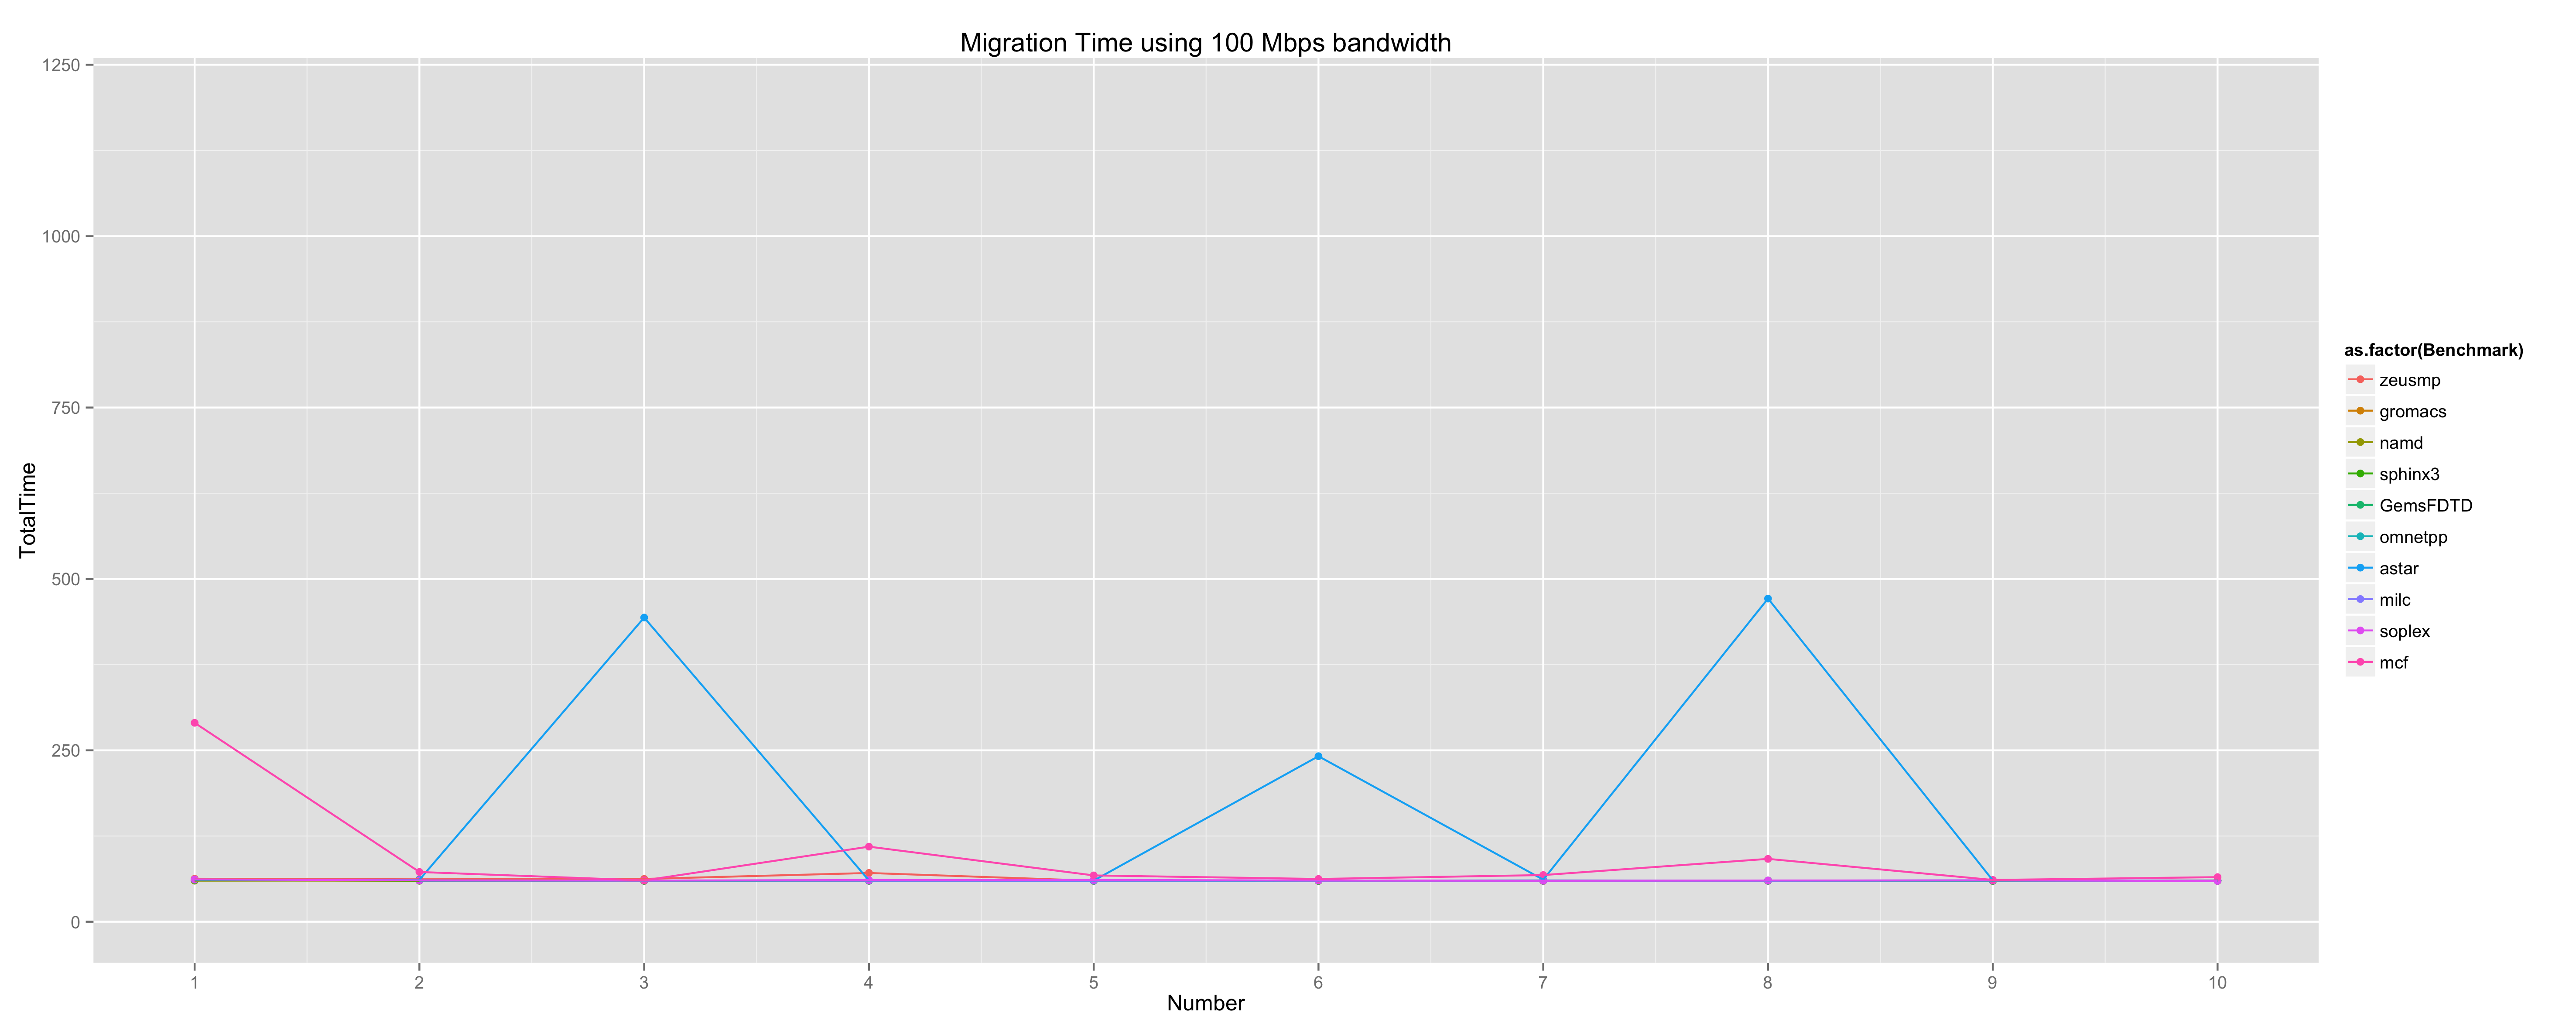
\includegraphics[width=400px]{migration_time100.png}\\ 
\caption{Time taken for Migration of VM}
\end{figure}

\subsection{Multiple Linear Regression Model for Migration Time}
Many variables observed in this experiments are related. The type of their relation can often be expressed in a mathematical form called Regression. Establishing and testing such a relation enables us :\\
1. To understand interactions, causes and effects among variables.\\
2. To predict unobserved variables on the basis of observed ones.\\
3. To determine which variables significantly affect the variable of interest.\\
Linear Regression model assumes that the conditional expectation \\
\begin{equation}
Y = G(x) = \beta_{0} + \beta_{1} x
\end{equation}
is a linear function of \(x\). As any linear function , it has an intercept \(  \beta_0 \) and a slope of \(  \beta_1 \).
A Multiple Linear Regression model assumes that the conditional expectation of a response: \cite{baron2013probability}
 \begin{equation}
Y = G(x) = \beta_{0} + \beta_{1} x^{(1)} + \beta_{2} x^{(2)} + ..... + \beta_{k} x^{(k)} 
\cite{baron2013probability}
\end{equation}
is a linear function of predictors \(  x^{(1)} , x^{(2)}  ,\ldots  ,x^{(k)}\). The intercept \( \beta_0 \) is the expected response when all the predictors equal to zero. The regression slope \( \beta_j \) is the expected change of the response \(Y\) when the corresponding predictor \(X^{(j)}\) changes by 1 while all the other predictor remain constant. 
Essentially in this experiment we collect a sample of \(n\) units and measured all \(k\) predictors on each unit such as Total L3 Miss, Mean CPU utilisation, Total Page Dirty,  Memory Access Rate, Total Instructions etc. on each unit. Also, the measured response variable Migration Time for each number of migration was recorded. The estimation of \(  \beta_1 , \beta_2, \ldots  ,\beta_k \) was realised using the method of least squares. \cite{baron2013probability} 
\\
Table-2 list all the variables considered for the multiple linear regression model.
\begin{table}[ht]
\caption{Various parameters considered for multiple linear regression model}
\begin{center}
    \begin{tabular}{ | l | | p{5cm} | p{5cm} |}
    \hline
    Name of the variable &  Description & Units \\ \hline
    TotalTime & Migration time for the benchmark and for a particular migration. & Seconds (Time). \\ \hline
    Bandwidth & Bandwidth used for the migration. & MBps.\\ \hline 
    TotalL3Miss & Total number of L3 Miss for the benchmark and for a particular migration. & L3 cache line misses in millions. \\ \hline
    TotalINST & Total number of instructions successfully retired by the CPU for  the benchmark and for a particular migration. & Number of instructions retired.\\ \hline
   MAR \cite{poellabauer2005feedback} &  \begin{equation}  TotalL3Miss/TotalINST  \end{equation} for the benchmark and for a particular migration. & L3Miss in millions per Number of instructions retired. \\ \hline
   MeanCpuUtilisation & Mean of CPU utilisation for the benchmark and for a particular migration. & Percent of CPU utilized. \\ \hline
   MemoryBandwidthUsed & \begin{equation}  Memory Used / Bandwidth  \end{equation} for the benchmark and for a particular migration. & MBps. \\ \hline
   TotalPageDirty, VM\_TotalPageDirty & Total number of Page dirtied for the benchmark and for a particular migration. Collected on host and VM. & Number of Pages. \\ \hline
  AvgROCL3M & Average Rate of change of L2 Misses. & L3 cache line misses in millions per Second. \\ \hline
  AvgROCPageDirty & Average Rate of change of page dirty. & Page dirtied per Second. \\ \hline
  PageDirtyPerSecondPerMigration & \begin{equation}  TotalPageDirty / TotalTime  \end{equation} for the benchmark and for a particular migration. & Page dirtied per Total Migration Time in Seconds. \\ \hline
    \end{tabular}
\end{center}
\label{tab:gt}
\end{table}
For this experiment, we have considered four models with different parameters from host machine and the VM. In this experiment, two sets of experiments were conducted, one for CPU intensive benchmarks and one for Memory intensive benchmarks. The dataset collected in the experiment was divided into two types, one for training and one for testing. Training set include all the migration time for the bandwidths 70, 80 and 90 Mbps. With the exclusion of the benchmarks zeusmp , GemsFDTD and milc in training set, due to the fact that the first migration took the entire execution time and for the rest of the nine migrations the VM was not running any load. Test set include all the migration time for the bandwidth 100 Mbps and for all benchmarks. Based on the Multiple Linear Regression Models, we predict the migration time for the Test dataset. Figure 4 (Model1) shows the regression model for the CPU intensive benchmark dataset without any parameters from the VM. Figure 5(Model2) shows the regression model for the Memory intensive benchmark dataset without any parameters from the VM. Figure 6(Mode3) and Figure 7(Model4) shows the regression model for the CPU intensive benchmark and Memory intensive benchmark datasets with total page dirtied from the VM. Considering Model1 for instance, the regression coefficient for TotalL3Miss and TotalINST  is \( 1.05 \times 10^{-7} \) and  \( 1.6 \times 10^{-4} \)  respectively, suggesting that an increase of 1 percent in TotalL3Miss and TotalINST is associated with a \( 1.05 \times 10^{-7} \) and  \( 1.6 \times 10^{-4} \) percent increase in the  Migration time, controlling for TotalINST, MAR and other parameters. Note that, for the CPU bound benchmarks the TotalPageDirty is also significant which is showed by \( p=0.00504 \). On the other hand, since this is model relates to CPU bound benchmark, the MAR is less significant and its not linearly related to Migration. Taken together the predictor variables account for around 99 percent of the variance in migration time for all the CPU intensive benchmarks. 
Figure 5 shows Model2, here the regression coefficient for TotalPageDirty  is \( 7.3  \times 10^{-1} \), suggesting that an increase of 1 percent in TotalPageDirty is associated with a \( 7.3 \times 10^{-1} \) percent increase in the Migration time, controlling for other parameters. Also, from the \(Pr(> |t|)\) column the interaction between MemoryBandwidthUsed and TotalPageDirty is significant. These results shows that, the parameter we considered can be used to explain the behaviour of our experiment. Taken together the predictor variables account for around 99 percent of the variance in Migration Time for all the Memory intensive benchmarks. Figure 6 and Figure 7 shows the Model3 and Model4, which include parameters like VM\_TotalPageDirty, interaction between MemoryBandwidthUsed with TotalPageDirty and interaction between MemoryBandwidthUsed and MAR. From Model3, the regression coefficient for VM\_TotalPageDirty is less significant. But for Model4 the regression coefficient for VM\_TotalPageDirty is very significant and also the interaction between MemoryBandwidthUsed and MAR. All together, the models explain the data with predictor variables account for around 99 percent of the variance in migration time.\\
Using the Test dataset, we intended to predict the migration time for CPU and Memory intensive benchmarks migrated under 100 Mbps bandwidth. The results for the predictions are shown in Figure 12-15. These figures shows the Benchmark name, actual time measure as TotalTime, Number as the migration, Predicted as values predicted from the model, and Error which is a difference between actual value and predicted value. The SquaredError column is the square of Error column, this is need to calculate the standard error as required by ordinary least squares(OLS).
\begin{figure}[h]
\centering
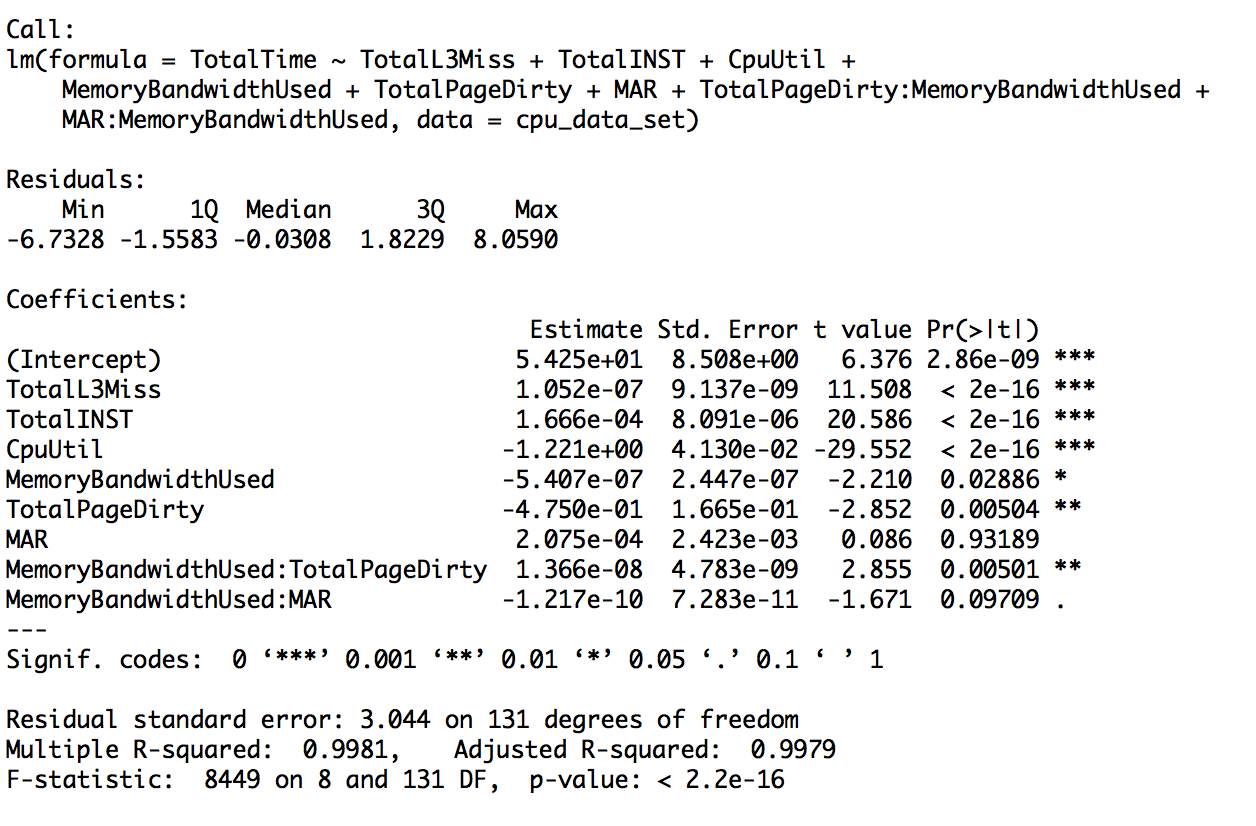
\includegraphics[width=250px]{CPU_MODEL} 
\caption{Mode1:Multiple Linear Regression Model for CPU intensive benchmark without parameters from VM}
\end{figure}
\begin{figure}[h]
\centering
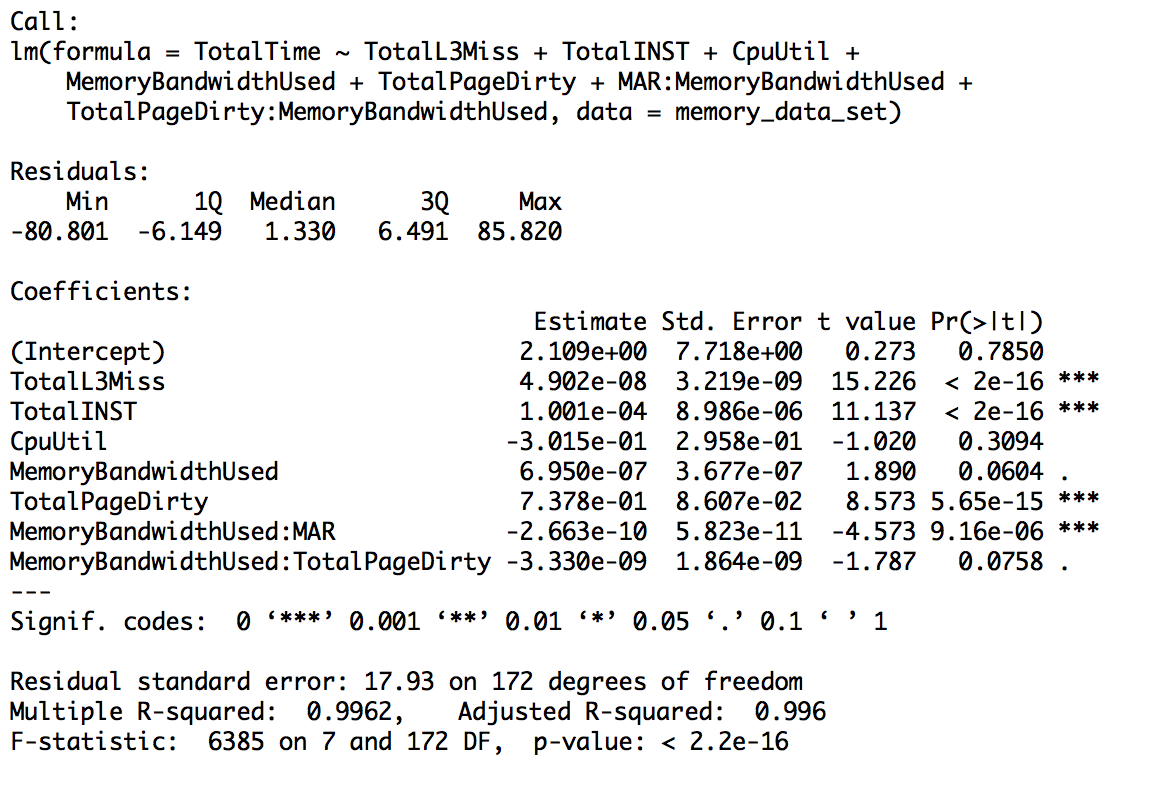
\includegraphics[width=250px]{MEMORY_MODEL} 
\caption{Model2:Multiple Linear Regression Model for Memory intensive benchmark without parameters from VM}
\end{figure}
\begin{figure}[h]
\centering
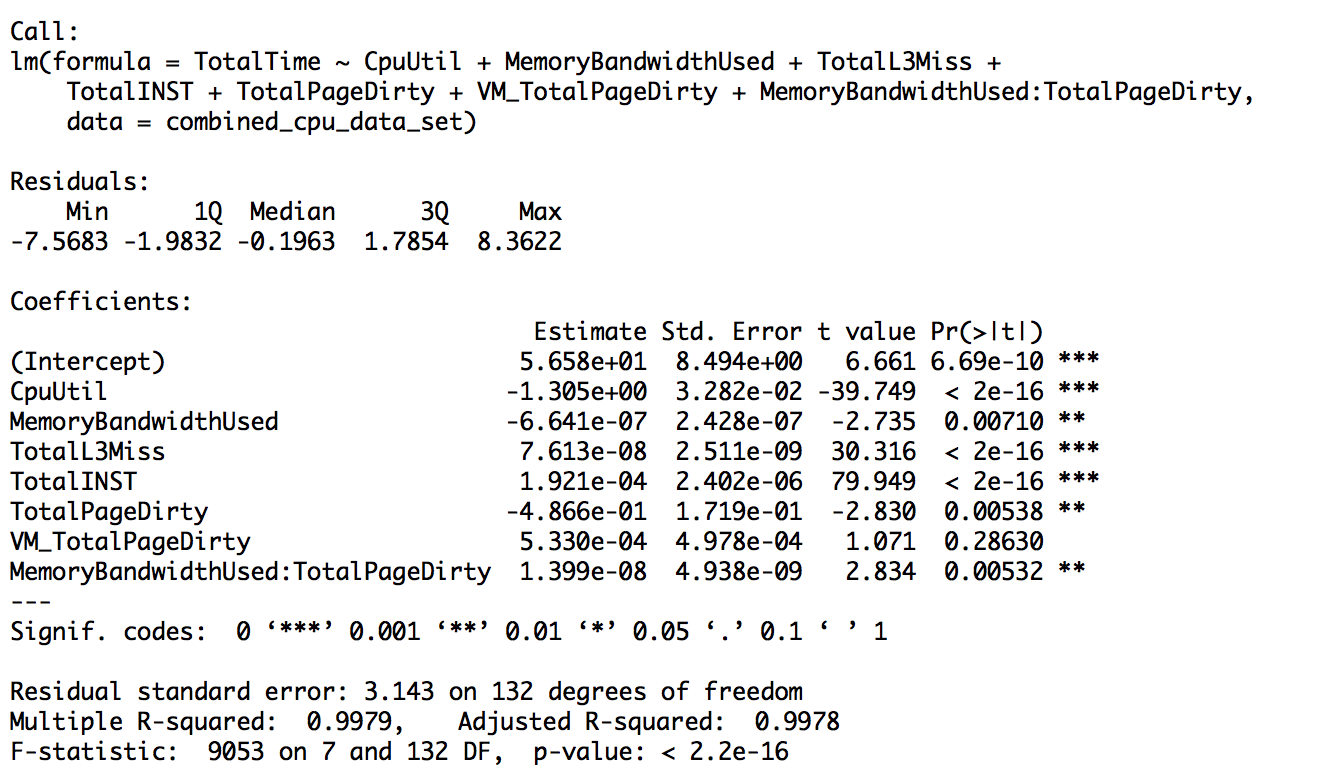
\includegraphics[width=250px]{CPU_COMBINED_MODEL} 
\caption{Model3:Multiple Linear Regression Model for CPU intensive benchmark with parameters from VM}
\end{figure}
\begin{figure}[h]
\centering
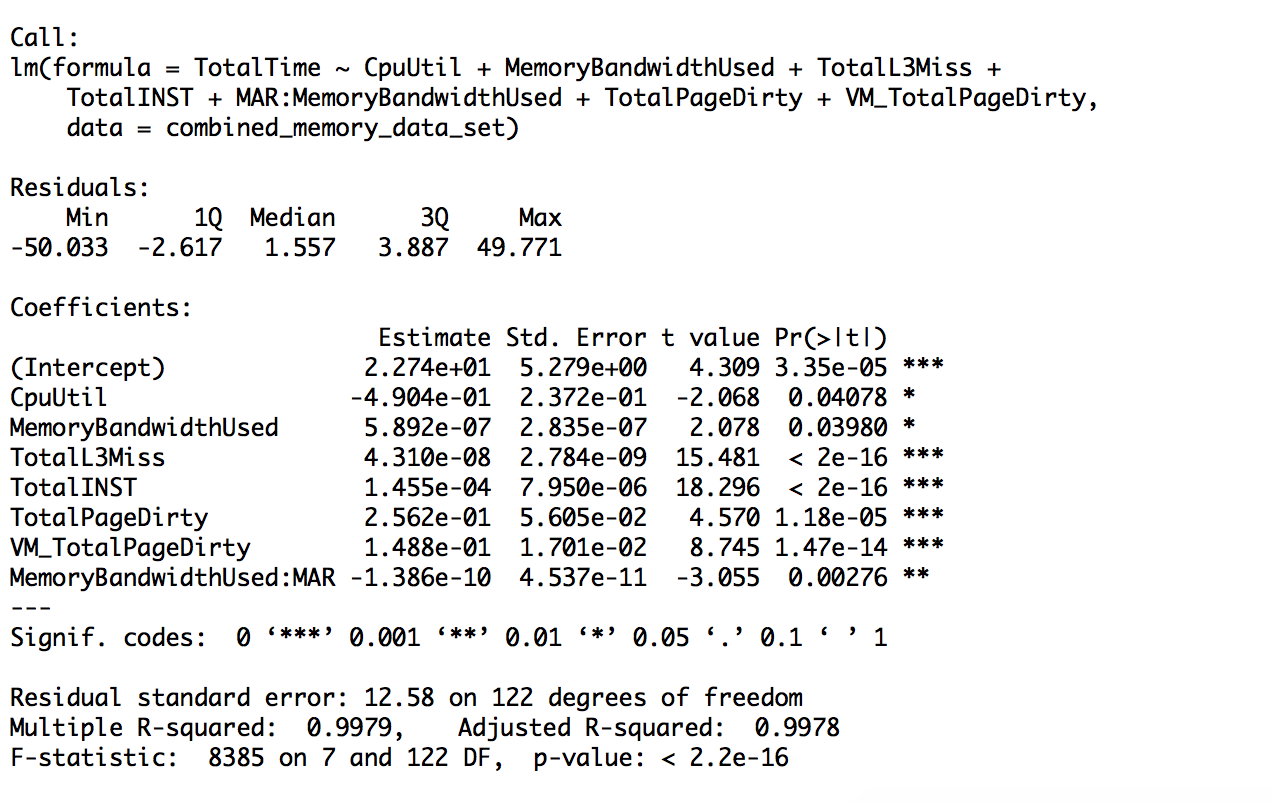
\includegraphics[width=250px]{MEMORY_COMBINED_MODEL}
\caption{Model4:Multiple Linear Regression Model for Memory intensive benchmark with parameters from VM}
\end{figure}
\section{Evaluation}
To evaluate the statistical assumptions underlying the models which is built using regression analysis. Four graphs that are useful for evaluating the model fit. Figure 8-11 \cite{kabacoff2011r} shows the Diagnostic plots for the four models considered in this study. With the assumptions from OLS regression we can understand these graphs. Normal Q-Q plot, which is in the upper left hand side, is a probability plot of the standardised residual against the values that would be expected under normality. All the four models the dependent variable is normally distributed for a fixed set of predictor values and the residual values are normally distributed with a mean close to 0. The Residual vs Fitted graphs captures all the systematic variance present in the data, leaving nothing but random noise. Apart from Model2, all models show clearly that Residual vs Fitted is curved  relationship. From the Figure-9 Residual vs Fitted graph suggest that we can add a quadratic term to the regression. \\
To evaluate the prediction accuracy, we need to calculate the standard error of the estimate. The regression model estimates that minimises the sum of squared deviations of prediction. The standard error of the estimate is closely related to this quantity and is defined \footnote{http://onlinestatbook.com/2/regression/accuracy.html} as:  
\begin{equation}
\sigma_{est} = \sqrt{\Sigma(actual value - predicted value) / total number of samples}
\end{equation}
The standard error of the estimate from all four models is given in Table-3. From the table, there is a tight fit for Model1 and Model3 suggesting that the predication valued are as close to actual values. Since the Model1 and Model3 are used for CPU intensive benchmark dataset, its evident that we can consider these models for prediction of migration time. In Model2 and Model4, which is the models for Memory Intensive benchmark dataset, has high sum of the squared errors when compared with other two models. As we can see from predicted data from Figure 13 and Figure 15, the predicted values are not too large compared to actual data. The high values for sum of the squared errors for models Model2 and Model4 can also be explained from the nature of the benchmark itself. As explained by \cite{jaleel2010memory} these benchmarks generate load in different time of the its execution time. 
\begin{table}[ht]
\caption{The standard error of the estimate from all four models}
\begin{center}
    \begin{tabular}{ | l | | p{5cm} | }
    \hline
    Model &  standard error of the estimate \\ \hline
    Model1 & 2.98426 \\ \hline
    Model2 & 22.86872 \\ \hline
    Model3 & 3.172431 \\ \hline
    Model4 & 29.60733 \\ \hline
    \end{tabular}
\end{center}
\label{tab:gt}
\end{table}
\begin{figure}[h]
\centering
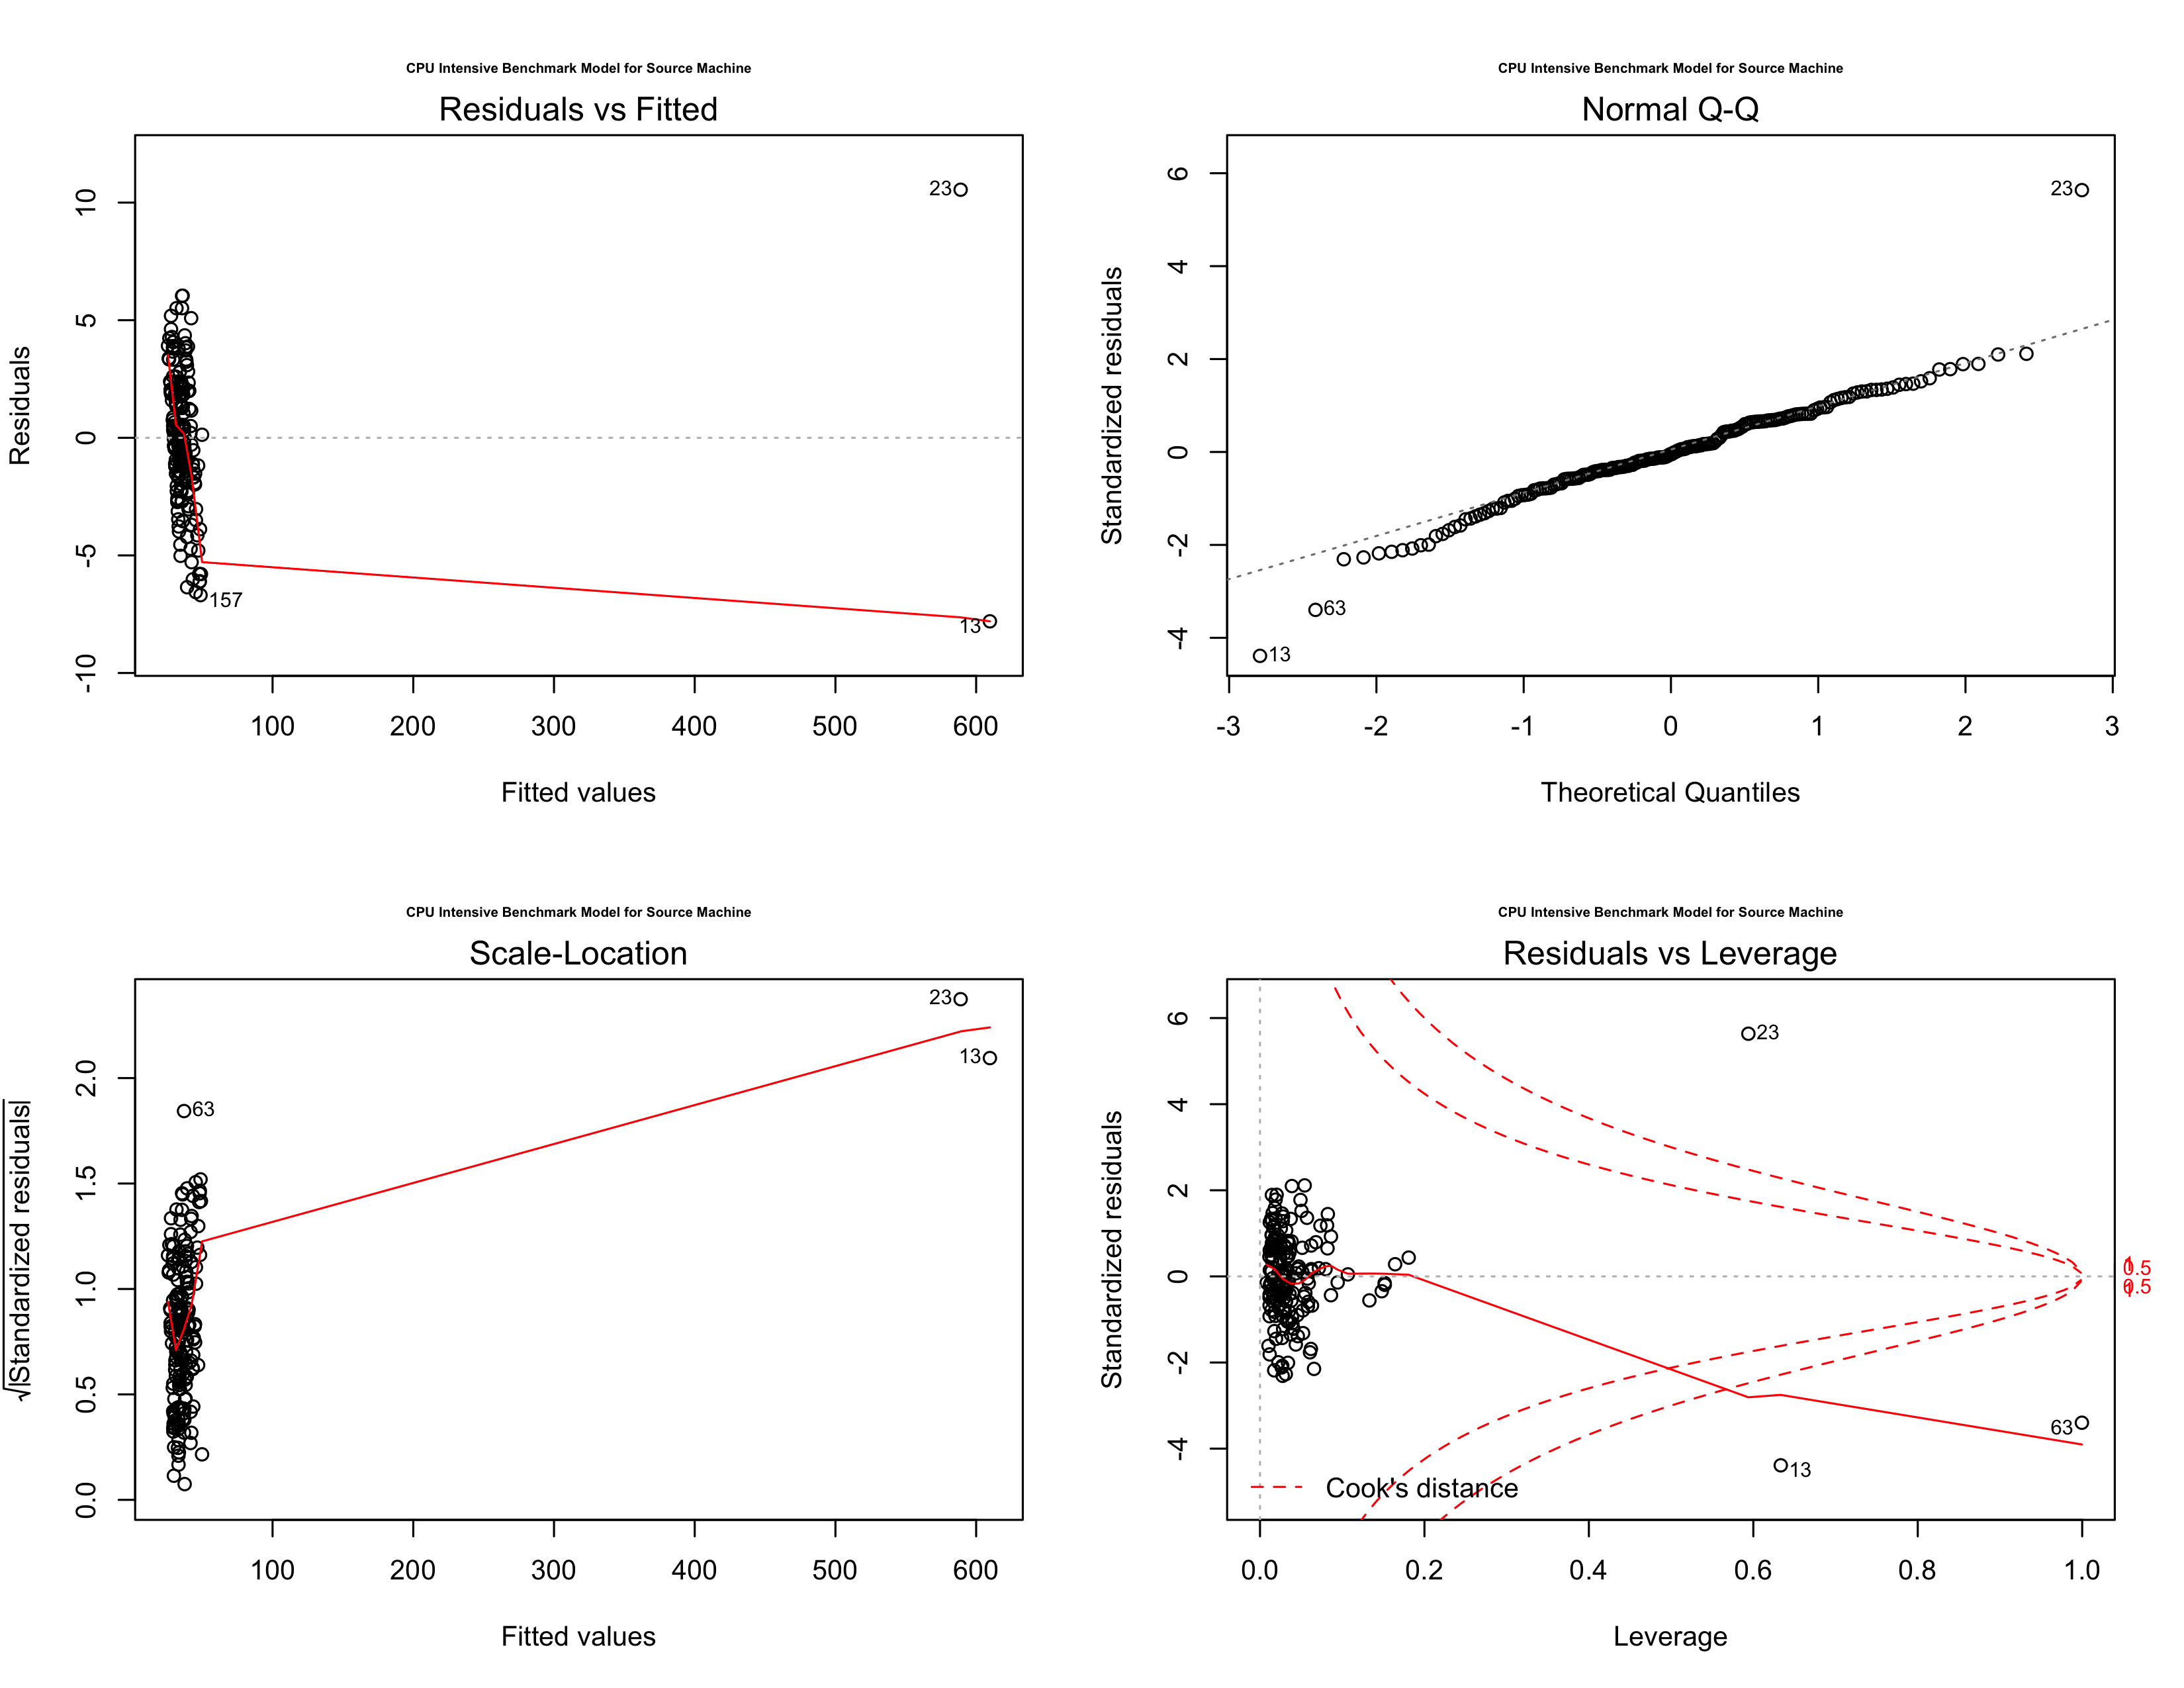
\includegraphics[width=400px]{source_model_cpu_intensive_benchmark.png} 
\caption{Model1:Diagnostic plots for Multiple Linear Regression Model for CPU intensive benchmark without parameters from VM}
\end{figure}
\begin{figure}[h]
\centering
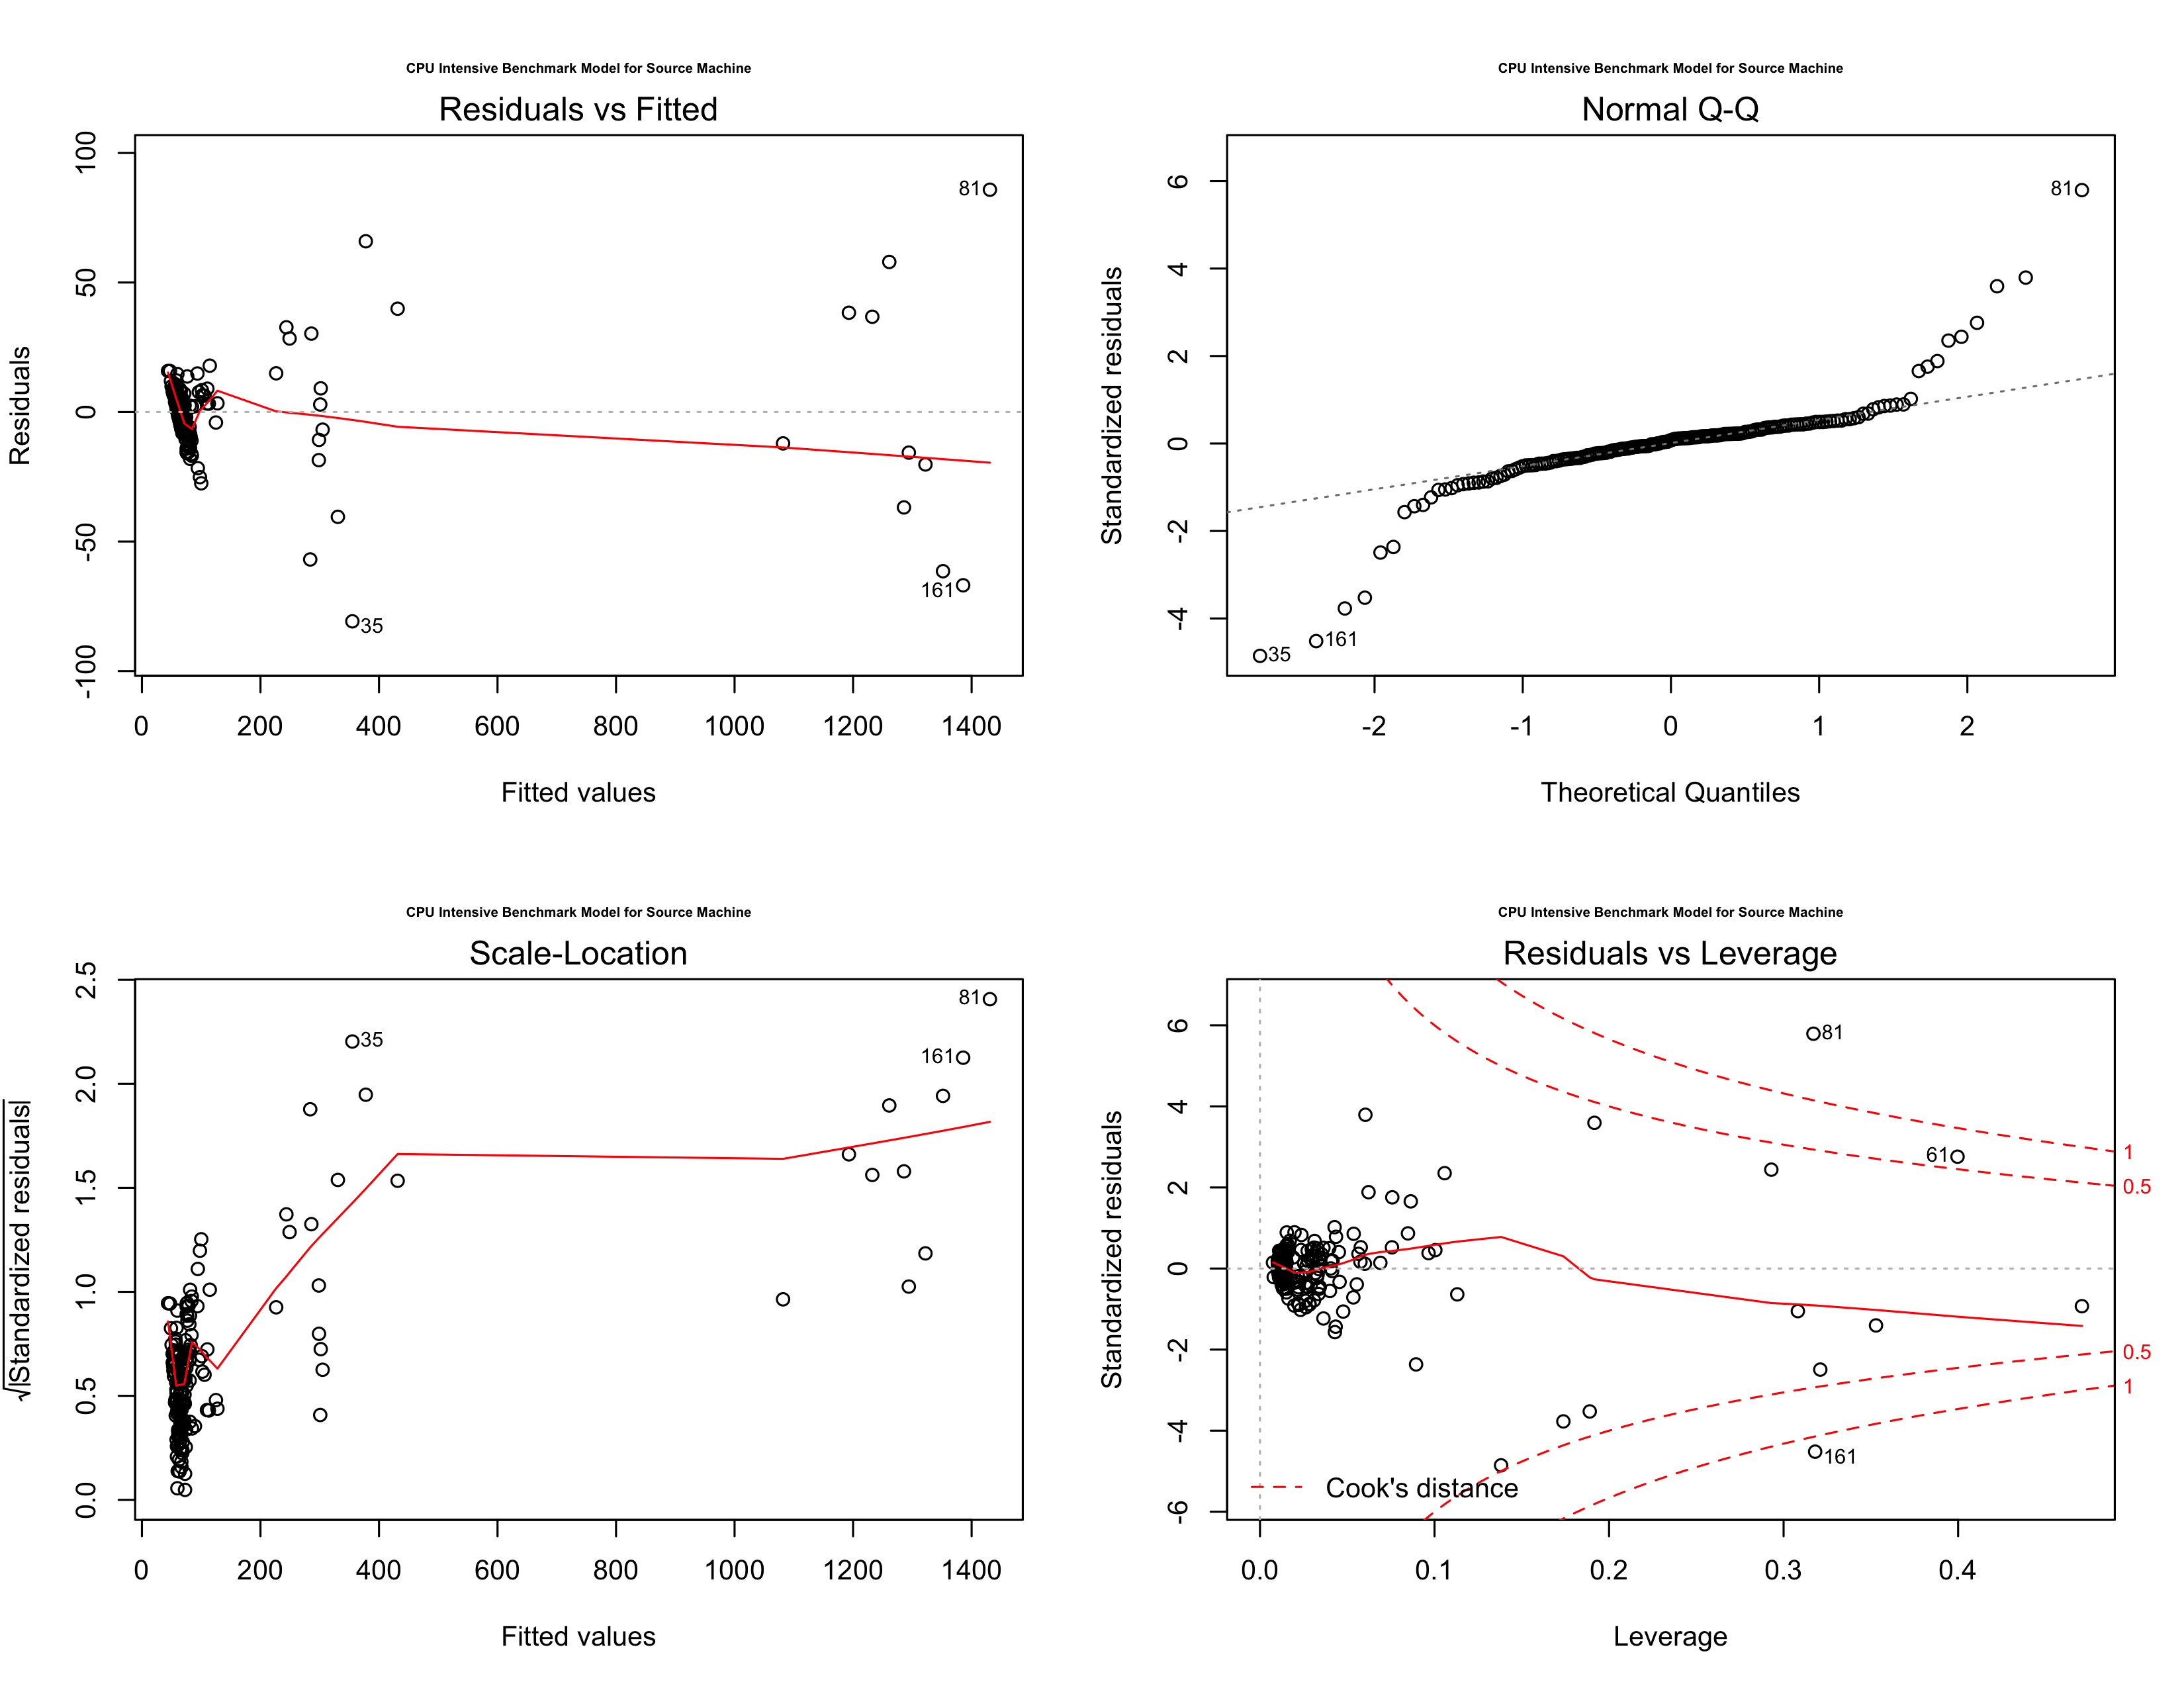
\includegraphics[width=400px]{source_model_memory_intensive_benchmkark.png} 
\caption{Model2:Diagnostic plots for  Multiple Linear Regression Model for Memory intensive benchmark without parameters from VM}
\end{figure}
\begin{figure}[h]
\centering
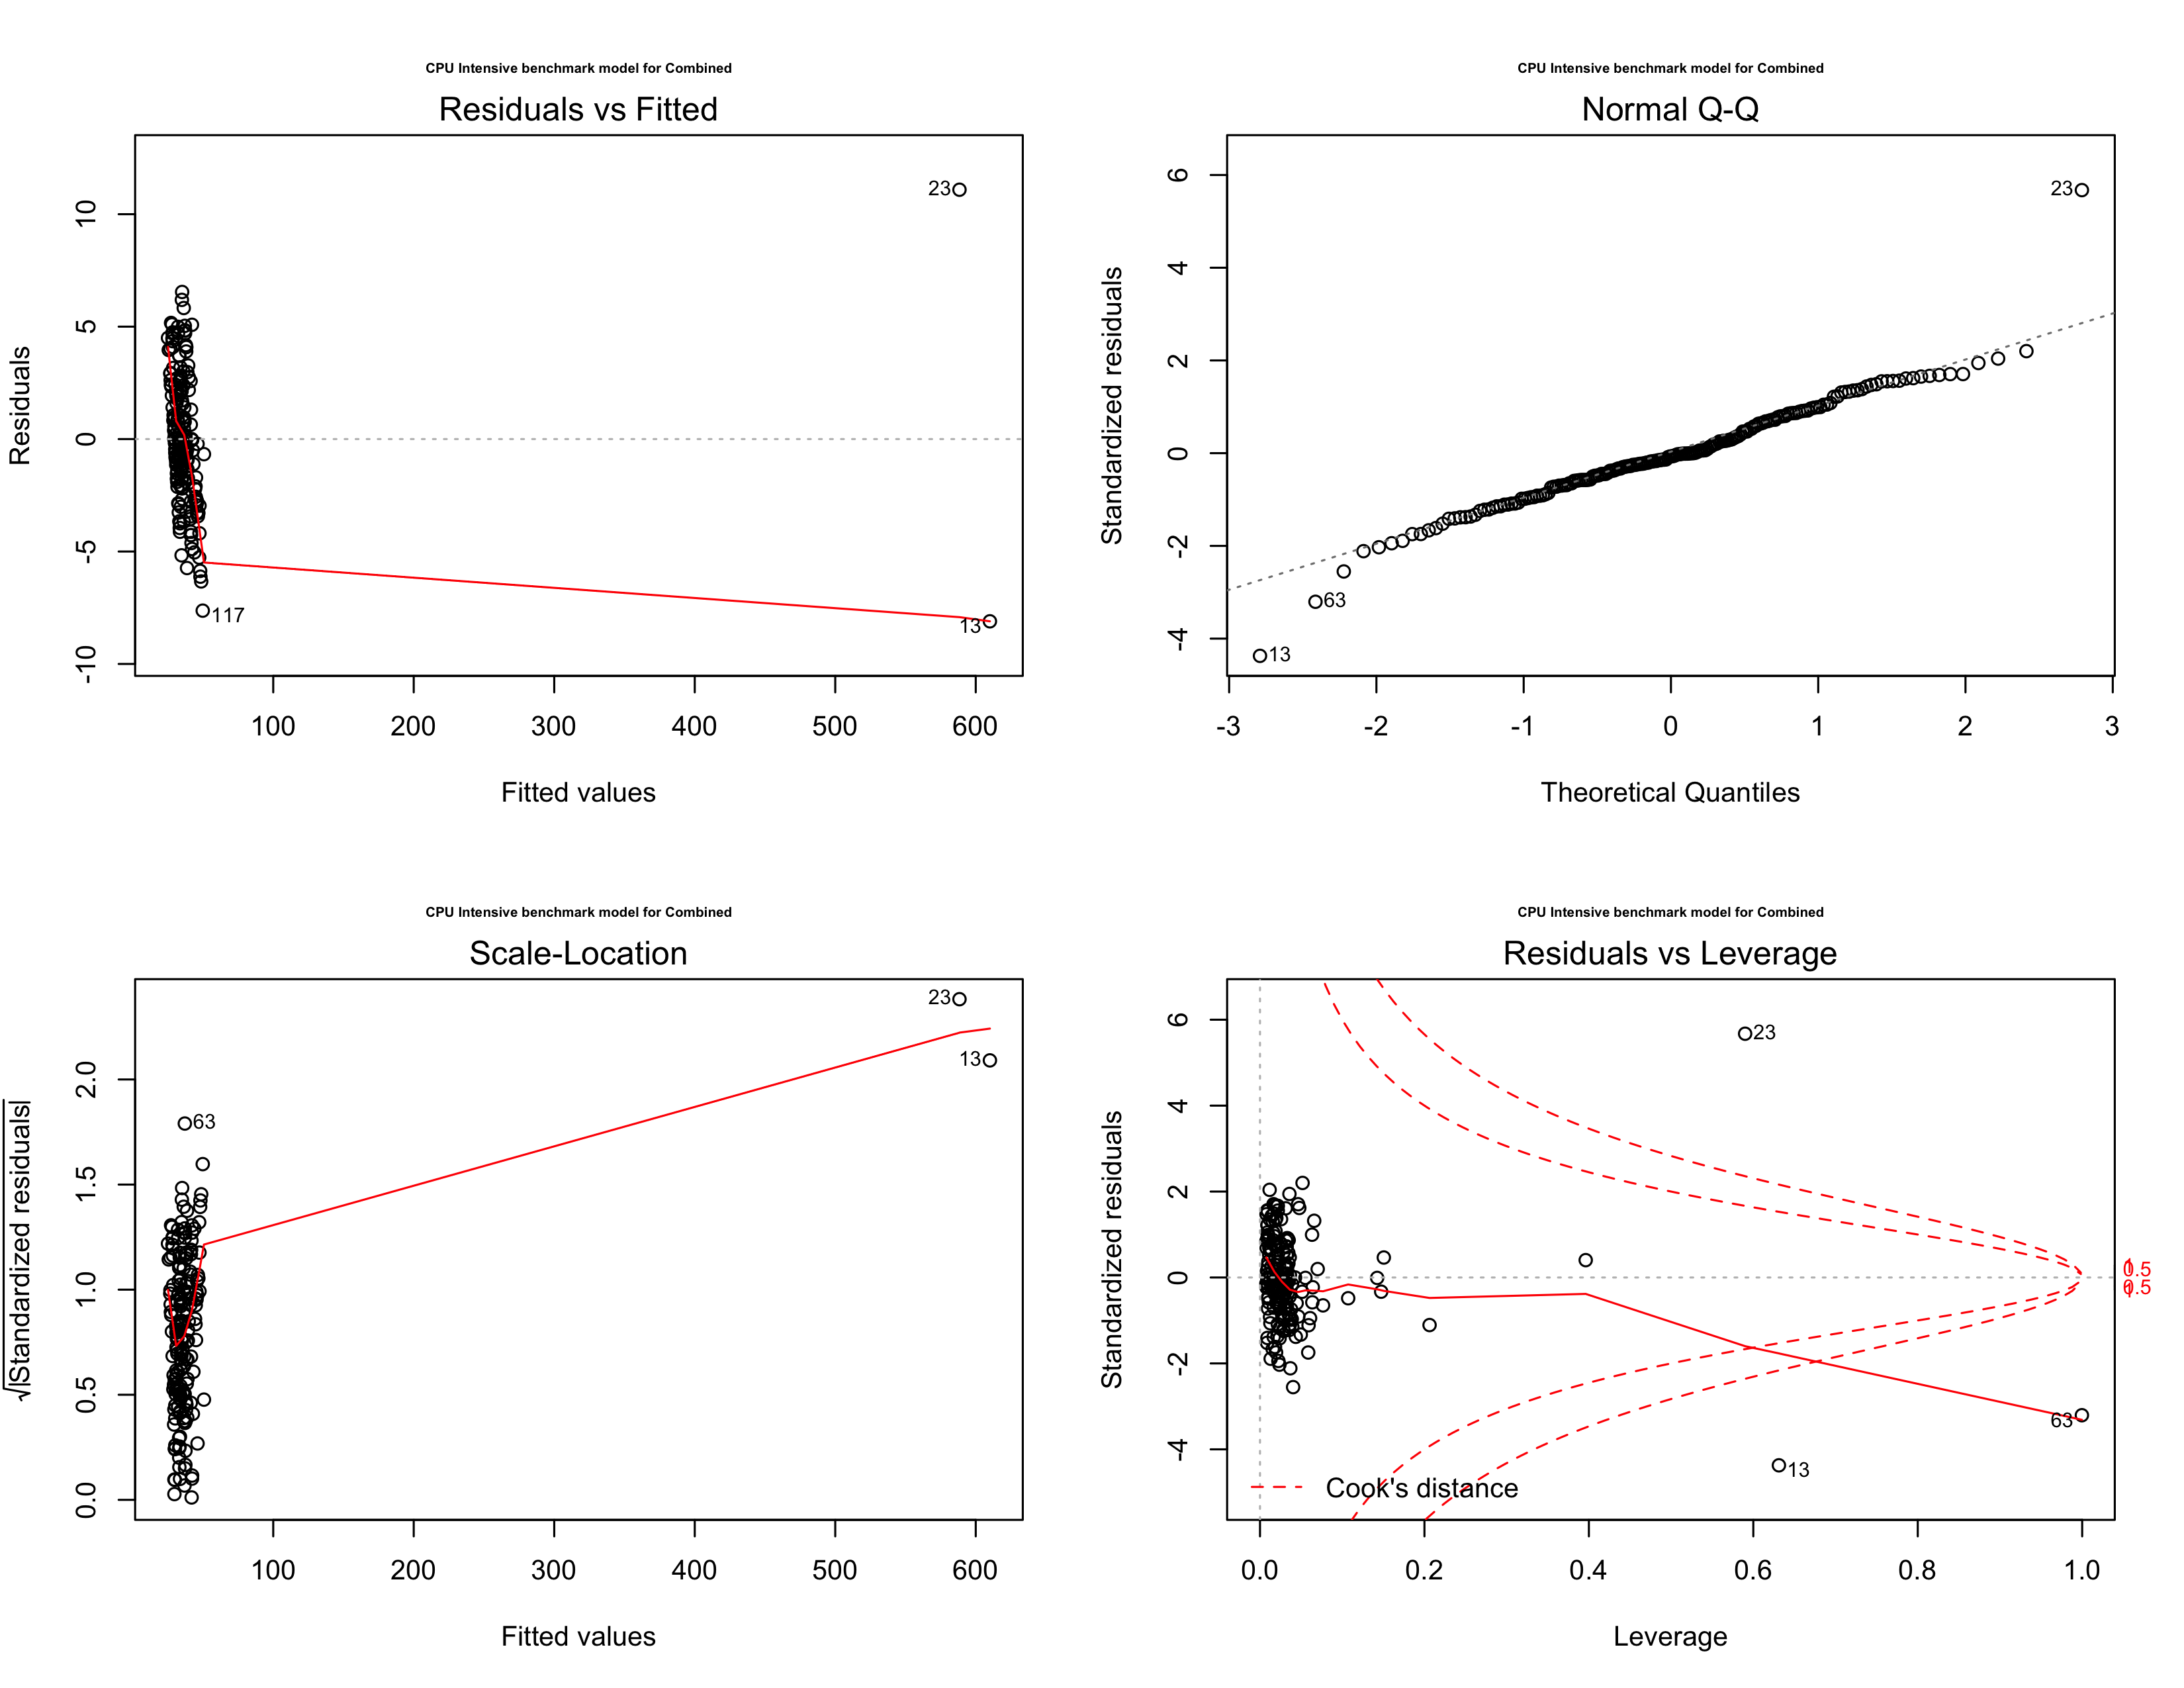
\includegraphics[width=400px]{combined_cpu_intensive_benchmark.png} 
\caption{Model3:Diagnostic plots for Multiple Linear Regression Model for CPU intensive benchmark with parameters from VM}
\end{figure}
\begin{figure}[h]
\centering
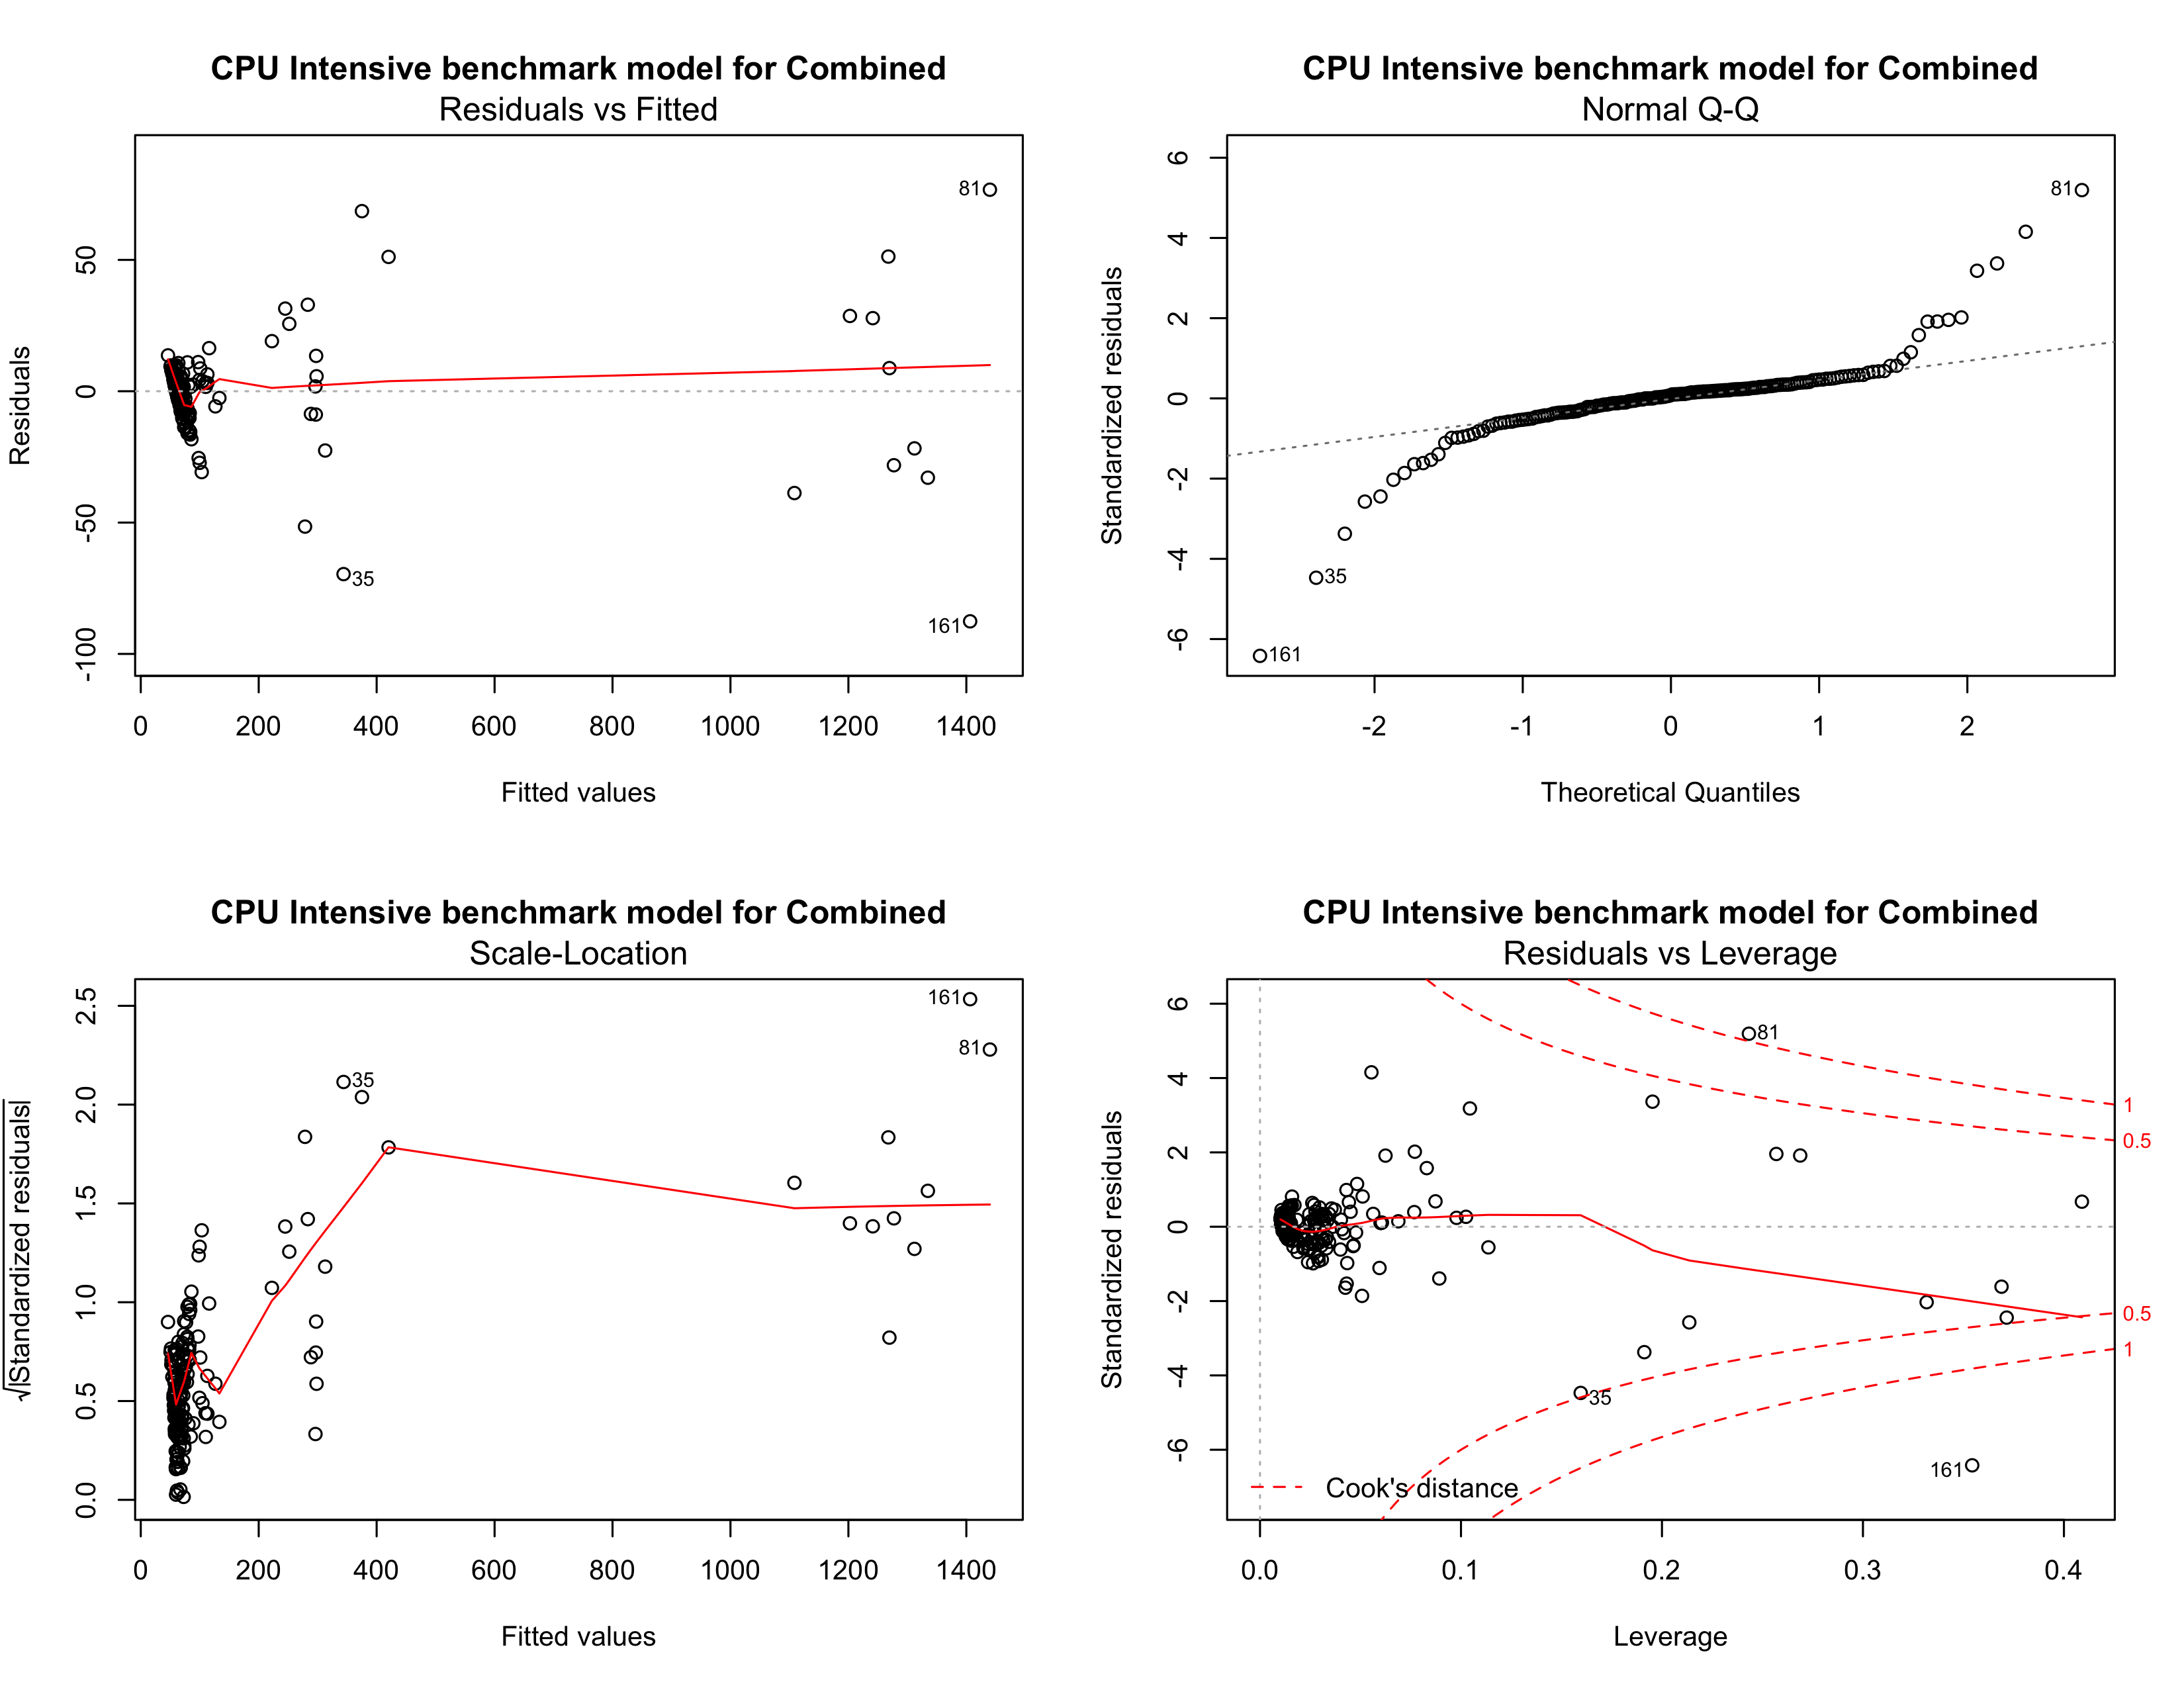
\includegraphics[width=400px]{combined_model_memory_intensive_benchmkark.png} 
\caption{Model4:Diagnostic plots for  Multiple Linear Regression Model for Memory intensive benchmark with parameters from VM}
\end{figure}
\begin{figure}[h]
\centering
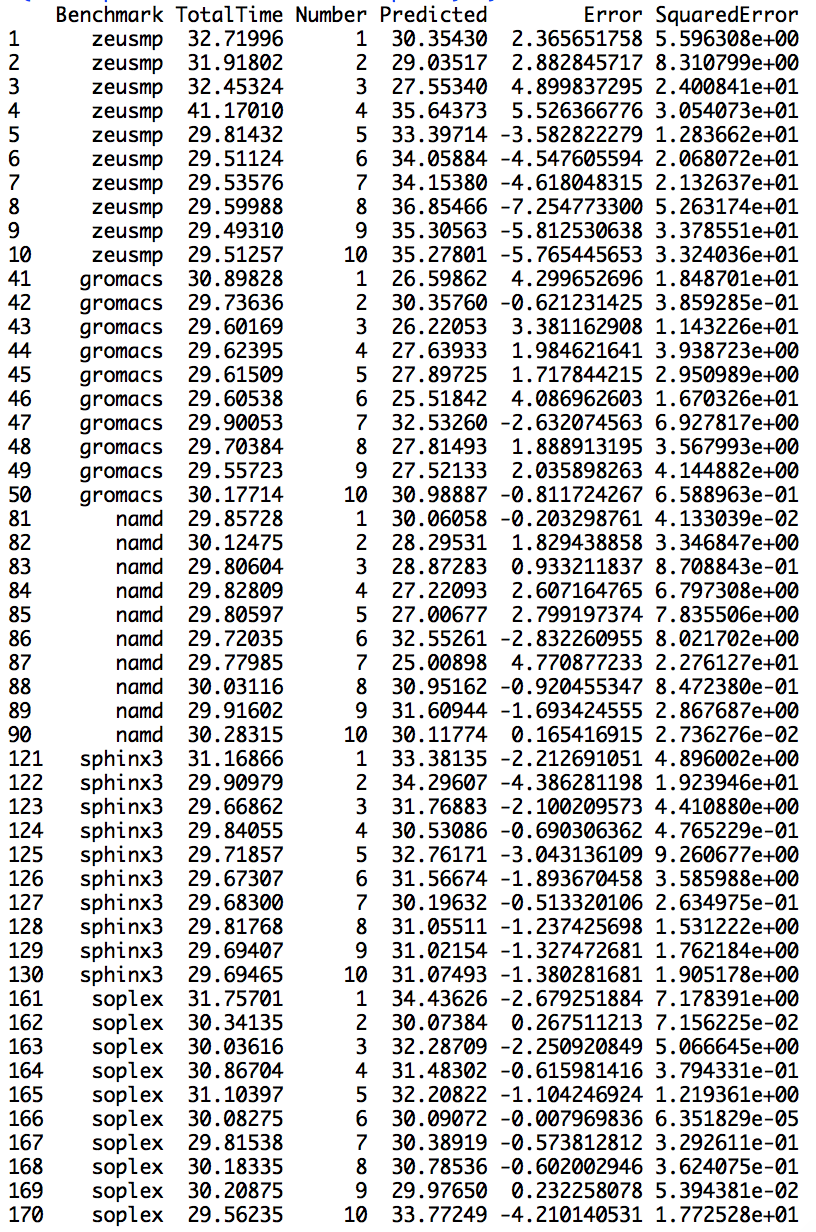
\includegraphics[width=400px]{pred1.png} 
\caption{Predictions from Model1}
\end{figure}
\begin{figure}[h]
\centering
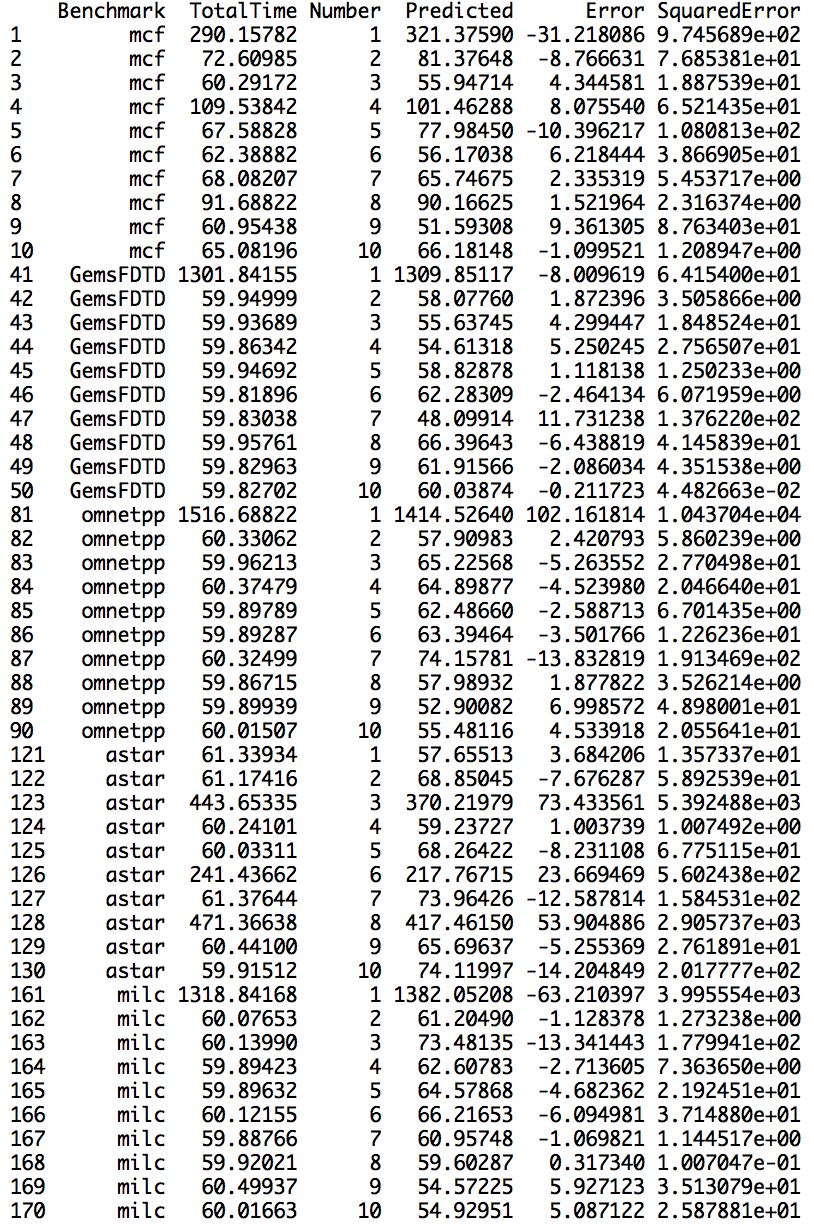
\includegraphics[width=400px]{pred2.png} 
\caption{Predictions from Mode2}
\end{figure}
\begin{figure}[h]
\centering
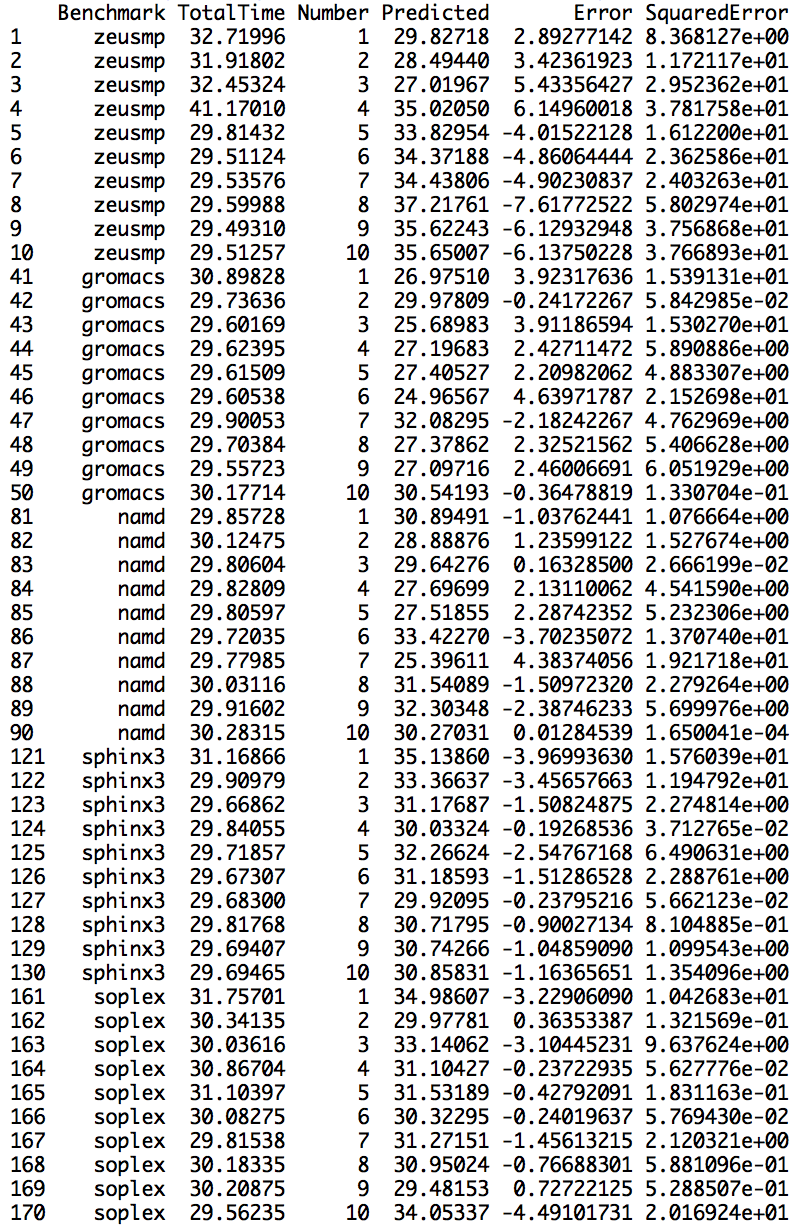
\includegraphics[width=400px]{pred3.png} 
\caption{Predictions from Model3}
\end{figure}
\begin{figure}[h]
\centering
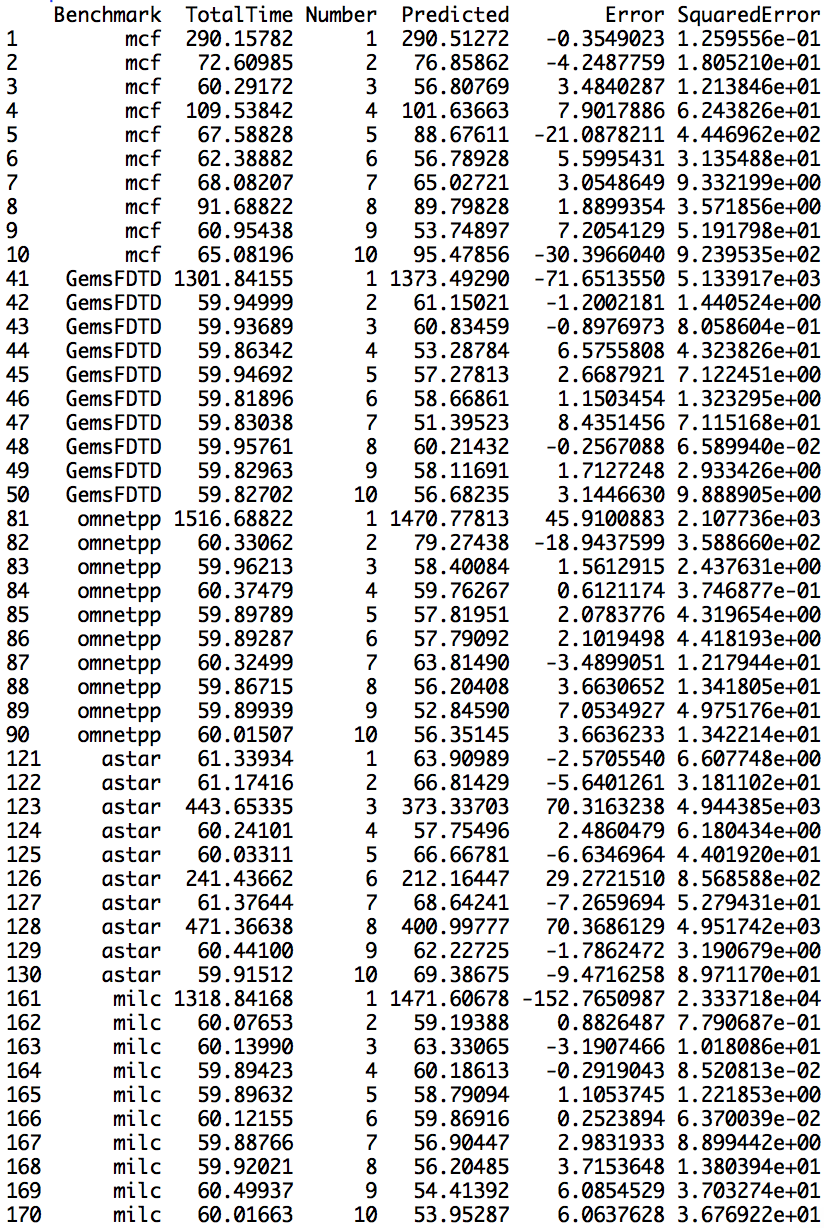
\includegraphics[width=400px]{pred4.png} 
\caption{Predictions from Model4}
\end{figure}
\section{Conclusion and Future Work}
In this internship, I investigate how various system resource (modelled as random variables) consumption can be used to estimate the VM migration time. Various other modelling technique have already suggested by \cite{liu2013performance}. But, under the guidance  of my supervisor, I showed that the migration time can estimated and analysed by using Multiple Linear Regression model with various predictors. Based on the models produced, these models can be used to predict the migration time. The concepts suggested by the supervisor was proves that the migration time can be estimated and predicted using the various parameters like page dirty rate, last level cache misses, RAM utilisation, network bandwidth and Memory access rate. SPECCPU2006 benchmark has 19 different benchmark tests, and more benchmarks for investigation is kept for future work. To conclude, we see a high potential the linear regression models presented and can be use to estimate and predict the migration time.
\bibliographystyle{ieeetr}
\bibliography{handin} 
\end{document}
